\documentclass{sig-alternate-10pt}
%\documentclass[10pt]{sigalternate052015}

\usepackage{amsmath}
\usepackage{amssymb}
\usepackage{xcolor}
\usepackage{url}
\usepackage{times}
\usepackage{xspace}
\usepackage{listings}
\usepackage{code}
\usepackage{algorithm}
\usepackage[noend]{algpseudocode}
\usepackage{tikz}
\usetikzlibrary{arrows,automata,positioning}
\let\proof\relax
\let\endproof\relax
\usepackage{amsthm}
\usepackage{subcaption}
\usepackage{balance}
\usepackage[ampersand]{easylist}
\usepackage{textcomp}
\usepackage{pifont}
\newcommand{\cmark}{\ding{51}}
\newcommand{\xmark}{\ding{55}}

\definecolor{princetonorange}{RGB}{255,143,0}
\definecolor{tmlblue}{RGB}{0,58,120}  % tmlblue == Toronto Maple Leafs Blue!

\newcommand{\todo}[1]{\textcolor{red}{[TODO: #1]}}
\newcommand{\ratul}[1]{\textcolor{blue}{[ratul: #1]}}
\newcommand{\ryan}[1]{\textcolor{green}{[ryan: #1]}}
\newcommand{\dpw}[1]{\textcolor{tmlblue}{[dpw: #1]}}
\newcommand{\todd}[1]{\textcolor{princetonorange}{[todd: #1]}}

\newcommand{\EG}{\emph{e.g.}}
\newcommand{\IE}{\emph{i.e.}}
\newcommand{\ETC}{\emph{etc.}}
\newcommand{\ETAL}{\emph{et al.}}

\newcommand{\sysname}{{\small \sf Methane}\xspace}
\newcommand{\sysnamesec}{{\sf Methane}\xspace}

\newcommand{\para}[1]{\paragraph*{\textbf{#1}}}

\newcommand{\set}[1]{\ensuremath{\{ #1 \} }}
\newcommand{\abs}[1]{\ensuremath{ \lvert #1 \rvert }}

\newcommand{\CD}[1]{\texttt{\small #1}}  % code font
\newcommand{\KW}[1]{\texttt{\small\bfseries{#1}}}

\newcommand{\True}{\CD{true}}
\newcommand{\Define}{\KW{define}}
\newcommand{\Prefer}{\texttt{>>}}
\newcommand{\Path}{\texttt{=>}}
\newcommand{\Link}{\texttt{->}}
\newcommand{\Agg}{\KW{agg}}
\newcommand{\Any}{\KW{any}}
\newcommand{\None}{\KW{drop}}
\newcommand{\In}{\KW{in}}
\newcommand{\Out}{\KW{out}}
\newcommand{\AND}{\texttt{\&}}
\newcommand{\OR}{\texttt{|}}
\newcommand{\NOT}{\texttt{!}}
\newcommand{\Intersect}{\ensuremath{\cap}}
\newcommand{\Union}{\ensuremath{\cup}}

\newcommand{\Exit}{\KW{exit}}
\newcommand{\End}{\KW{end}}
\newcommand{\Start}{\KW{start}}
\newcommand{\Enter}{\KW{enter}}
\newcommand{\Eventually}{\KW{eventually}}
\newcommand{\Already}{\KW{already}}
\newcommand{\Internal}{\KW{internal}}
\newcommand{\Never}{\KW{never}}
\newcommand{\Always}{\KW{always}}
\newcommand{\Through}{\KW{through}}
\newcommand{\LinkKW}{\KW{link}}
\newcommand{\PathKW}{\KW{path}}
\newcommand{\Novalley}{\KW{novalley}}

\renewcommand{\path}[2]{ #1 \mapsto \ensuremath{#2} }

%% grammar
\newcommand{\BNFALT}{\;\;|\;\;}
\newcommand{\hdr}[2]{\flushleft \chdr{\hspace{5mm}#1}{#2}}
\newcommand{\chdr}[2]{\textbf{#1} {#2} \\ \centering}%


\begin{document}

%\CopyrightYear{2016}
%\setcopyright{acmcopyright}
%\conferenceinfo{SIGCOMM '16,}{August 22-26, 2016, Florianopolis , Brazil}
%\isbn{978-1-4503-4193-6/16/08}\acmPrice{\$15.00}
%\doi{http://dx.doi.org/10.1145/2934872.2934909}

\special{papersize=8.5in,11in}
\setlength{\pdfpageheight}{\paperheight}
\setlength{\pdfpagewidth}{\paperwidth}

\title{An Abstraction-based Approach to Network Synthesis}

%\author{Paper \#324, 14 pages}


\author{%
Ryan Beckett\\
  \affaddr{Princeton}
  %\\
  %\email{rbeckett@princeton.edu}
\and
Ratul Mahajan\\
  \affaddr{Microsoft}
  %\\
  %\email{ratul@microsoft.com}
\and
Todd Millstein\\
  \affaddr{UCLA}
  %\affaddr{University of California, Los Angeles}
  %\\
  %\email{todd@cs.ucla.edu}
\and
Jitendra Padhye\\
  \affaddr{Microsoft}
  %\\
  %\email{padhye@microsoft.com}
\and
David Walker\\
  \affaddr{Princeton}
  %\\
  %\email{dpw@princeton.edu}
}

\maketitle


%=====================================================
%
%
%  **Abstract**
%
%
%=====================================================


% Points to make
%
% (1) Lets operators think about topologies/policies at a high-level of abstraction
%     - matches current thinking (e.g., templates)
%
% (2) Promotes a correct-by-construction methodology
%
%     properties that hold over abstract topologies hold over concrete ones
%      - includes correct forwarding behavior
%      - includes reachability (under k-failures)
%
% (3) Enables reusability (e.g., across datacenters) and expansion (e.g., within a datacenter)
%
% (4) lets us scale synthesis to large-scale topologies


\textbf{Abstract---}
We develop techniques for automated reasoning about end-to-end properties of abstract network topologies. We extend a network synthesis tool, \sysname, to allow network operators to write a high-level routing policy over an abstraction of their network topology. From such a specification, \sysname synthesizes a collection router configurations running the distributed Border Gateway Protocol (BGP) that are guaranteed to implement the centralized routing policy for any concrete instantiation of the abstract topology, and for any combination of network failures in the resulting concrete topology.
%
Additionally, properties proven by \sysname over the abstract topology, such as reachability between a source and destination under k-failures, are also guaranteed to hold under any concrete instantiation of the abstract topology.
%
Something something, expandable/incremental networks. Something something scales compilation to large networks. Something something, templates easier to understand.
%These strong guarantees allow operators to reason about the routing behavior of their network at a high-level abstraction, while also generating an efficient low-level implementation.
%
%In addition, operators are able to safely change or expand their network in any way, so long as the new resulting topology also respects the abstraction.
%
We test \sysname out on ... blah blah blah



%=====================================================
%
%
%  **Keywords**
%
%
%=====================================================

%\vspace{0.1in}
%\noindent
%\textbf{CCS Concepts}\\
%$\bullet$ Networks $\rightarrow$ {\em Network control algorithms; Network reliability; Network management;}
%$\bullet$ Software and its engineering $\rightarrow$ {\em Automated static analysis; Domain specific languages}

%\vspace{0.1in}
%\noindent
%\textbf{Keywords}\\
%Propane; Domain-specific Language; BGP; Synthesis; Compilation; Fault Tolerance; Distributed Systems


%=====================================================
%
%
%  **Introduction**
%
%
%=====================================================


\section{Introduction}
\label{sec:introduction}

\begin{easylist}[itemize]
& Network configuration is difficult/error-prone. Operators think of policy at
  a high level of abstraction, yet for implementations:
&& Often configs must be decomposed device-by-device
&& Often need to create reusable configurations for different topologies/policies
&& Ensure different devices/networks kept consistent when policy changes

& Current state of the art is to capture abstractions using parameterized
  device templates. The same templates can then be reused across multiple
  devices. Unfortunately, existing template systems have many limitations
&& Templates often still require the operator to reason about network-wide
   policy device-by-device.
&& Templates do not provide any guarantees of configuration correctness,
   instead requiring the operator to manually reason about forwarding for
   any possible concrete network
&&& In addition, operators must reason about possible network failures that
    might arise in one concrete network versus another

& To this end, we build a language called \sysname to simplify the operators task.
&& \sysname allows the operator to define high-level network abstractions to reflect
   the operator's mental model, and then to write a centralized routing policy over the
   abstraction.
&& We extend the \sysname intermediate graph-based representation to support abstract policies,
   and show how to compile abstract \sysname policies to this representation.
&& As a major use-case, we show how the compilation and failure-safety analysis
   of the Propane configuration-synthesis tool can be extended over abstract topologies.
&& We develop an abstract interpretation that operates over this graph representation and verifies
   if properties, such as reachability or k-disjoint paths between two nodes, are guaranteed
   to hold for any possible concrete instantiation of the network.
&& Our major result is an abstraction theorem, which states that ...
&& The result is that policies compiled with the Propane compiler to distributed configurations
   are guaranteed to have correct forwarding behavior for any possible concrete instantiation
   of the network, and for any possible combination of failures in the given concrete network.
&&& Finally, we show how abstract compilation makes it possible to dramatically speed up compilation
    time for the Propane policies, cite some numbers here ...
\end{easylist}

% Some useful citations from the previous paper listed below

%It is well known that configuring networks is error
%prone and that such errors can lead to disruptive
%downtimes~\cite{mahajan+:bgp-misconfiguration,feamster+:rcc,batfish,dc-failure-study}.
%For instance, a recent misconfiguration led to an hour-long, nation-wide outage for Time Warner's backbone network~\cite{time-warner}; and a major BGP-related incident makes international news every few months~\cite{bgpmon}.%

%A fundamental reason for the prevalence of misconfigurations is the
%semantic mismatch between the intended high-level
%policies and the low-level configurations.
%Many policies involve network-wide properties---prefer a certain neighbor,
%never announce a particular destination externally,
%use a particular path only if another fails---but configurations describe the behavior of
%individual devices.
%%
%Operators must manually decompose network-wide policy into
%device behaviors, such that policy-compliant behavior results from the distributed interactions of
%these devices.
%%
%Policy-compliance must be ensured not only under normal
%circumstances but also during failures.  The need to reason
%about all possible failures exacerbates the challenge
%for network operators.  As a result, configurations that work
%correctly in failure-free environments have nonetheless been found to violate key
%network-wide properties when failures occur~\cite{batfish}.%

%To reduce configuration errors, operators are increasingly adopting an
%approach in which common tasks are captured as parameterized templates~\cite{hatch,thwack}.
%%
%While templates help ensure certain kinds of consistency across devices,
%they do not provide fundamentally different abstractions from existing configuration languages
%or bridge the semantic divide between network-wide policies and device-level configuration.
%Thus, they still require operators to
%manually decompose policies into device behaviors.%

%As a complementary approach, configuration analysis tools can help reduce misconfigurations by checking if low-level configurations match high-level policy~\cite{batfish,feamster+:rcc}. However, such tools cannot help operators with the challenging task of generating configurations in the first place.%

%Software-defined networking (SDN) and its abstractions
%are, in part, the research
%community's response to the difficulty of maintaining policy
%compliance through distributed device interactions~\cite{ethane}.
%Instead of organizing networks around a distributed
%collection of devices that compute forwarding tables through
%mutual interactions, the devices are told how to
%forward packets by a centralized controller. The controller is responsible for ensuring that the
%paths taken are compliant with operator specifications.%

%The centralized control planes of SDN, however, are not a panacea.
%First, while many SDN programming systems~\cite{sdn-languages} provide effective \emph{intra}-domain routing
%abstractions, letting users specify paths within their network,
%they fail to provide a coherent means to specify \emph{inter}-domain routes.
%Second, centralized control planes
%require careful design and engineering to be robust to failures---one must ensure that all devices can communicate with the controller at all times, even under arbitrary failure combinations. Even ignoring failures, it is necessary for the control system to
%scale to meet the demands of large or geographically-distributed networks,
%and to react quickly
%to environmental changes. For this challenge, researchers are exploring
%multi-controller systems with interacting controllers, thus bringing back distributed
%control planes~\cite{mccauley2013extending,onos} and their current programming difficulties.%


%=====================================================
%
%
%  **Motivation**
%
%
%=====================================================

\section{Motivation}
\label{sec:motivation}

\begin{figure}[t!]
  \centering
  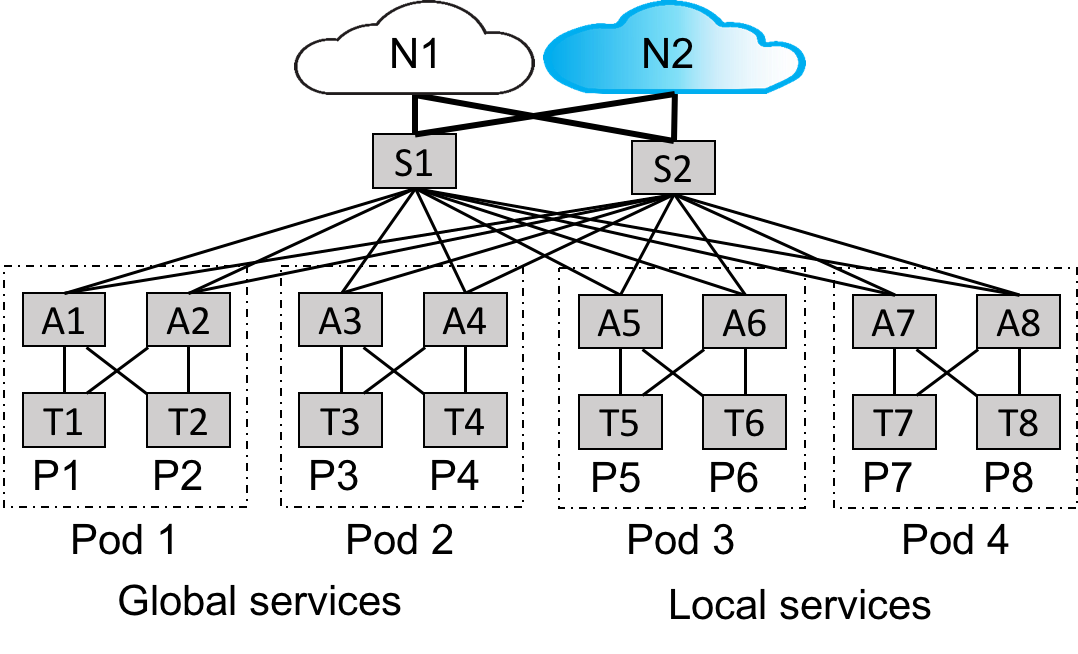
\includegraphics[width=2.5in]{figures/example}
  \caption{An example data center network.}
  \label{fig:example}
  \vspace{-1em}
\end{figure}

\begin{figure}[t!]
  \centering
  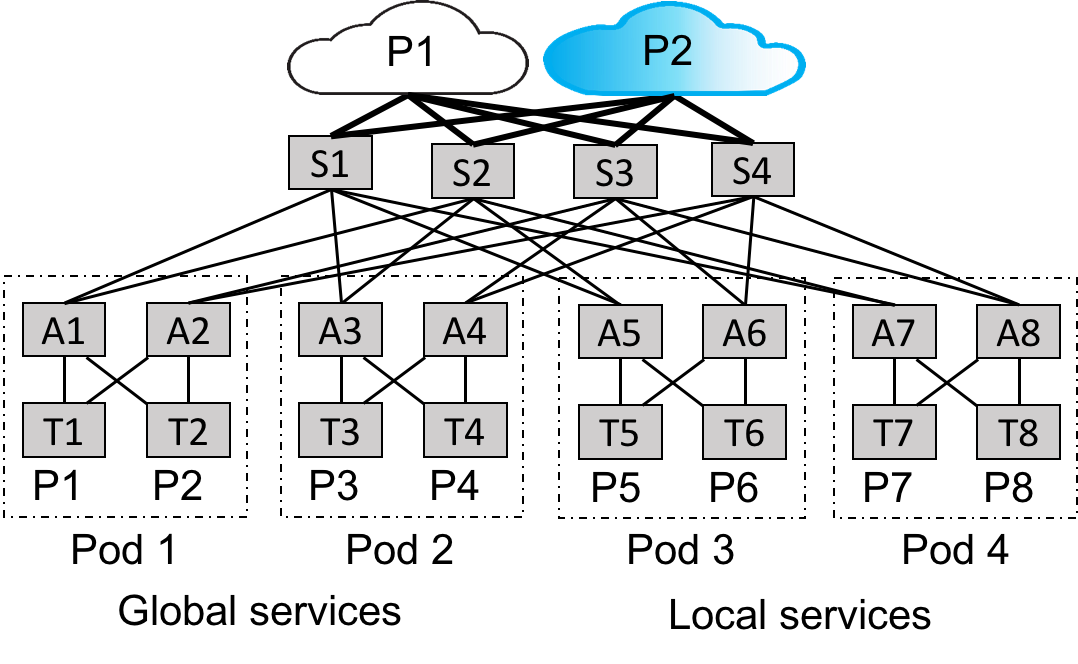
\includegraphics[width=2.5in]{figures/example2}
  \caption{A modified version of the example in Figure~\ref{fig:example}.}
  \label{fig:example2}
  \vspace{-1em}
\end{figure}

%We motivate \sysname using an example data center network. Our network, 
Consider the data center network shown in Figure~\ref{fig:example}.  The boxes in the diagram
represent \emph{switches}, and these switches play several different roles:  T[1--8] denote top-of-rack (ToR) switches, A[1--8] denote aggregation switches, and S[1--2] denote spine switches. The spine switches are connected to the
rest of the internet; any traffic to or from the outside world flows through them.  The aggregation switches
serve as a bridge between spine and ToR switches.   Finally, each ToR switch is
connected to a set servers (``a rack''): P[1--8] denote groups of addresses for services hosted in each rack. Such groups are called address {\em prefixes} because they are encoded using the adresses' shared prefix. 

We assume that each switch is running an instance of the \emph{Border Gateway Protocol} (BGP), 
as is common in large data centers. In this protocol, adjacent switches use BGP to exchange messages
with one another concerning the availability of routes to destinations.  A BGP \emph{configuration}
(one for each switch) dictates which offered routes a switch will select and how to propagate chosen routes to its 
neighbours.\footnote{If this submission is accepted and more space is available in the final version, 
we will give a detailed explanation of BGP for the PLDI audience.  Henceforth, we assume knowledge of basic BGP
mechanics.}

%Assume that all nodes are running the border gateway protocol (BGP), as is common in large data centers~\cite{x}. \todo{more detail on BGP?}

The intended high-level operator policy for this network is as follows. Internal connectivity should be complete, \IE, all nodes must be able to talk to each other. Services in Pods 1 and 2 should be globally accessible and thus their addresses should be announced externally, but only after aggregating individual prefixes P[1--4] into a single prefix PG. Finally, services in Pods 3 and 4 not should be externally visible and thus their address should not be announced externally.

To correctly configure the policy above, the network engineer's task is to generate low-level configurations for each switch in the network. This implies ensuring, for instance, that all switch interfaces are assigned correct addresses; all routing adjacencies are correctly configured (\EG, T1's configuration includes A1 as neighbor and vice-versa); all switches announce their own addresses (so that they can be reached for management purposes) and the ToRs announce the correct prefixes for their services; all switches  forward the prefix announcements that they should to each neighbor and not forward those that they should not (\EG, the spines should forward prefixes for local services to internal neighbors but not external neighbors); and the spines announce externally only the aggregate global prefix. \dpw{Do we need to explain aggregation here?}

As many have observed before, such configuration tasks are highly challenging. Consequently, configuration errors are the leading cause of network outages~\cite{juniper-study,bgpmon,batfish,propane}.

\subsection{Limitations of concrete synthesis}

In response, researchers have developed systems that synthesize low-level device configurations from high-level policy statements~\cite{narain:lisa05,narain+:configassure,dadc,propane}.
%They take network topology and policy as input and output device configurations that are  guaranteed to be correct under all possible failures. Thus, they save the engineers from performing the complex task of breaking down global policies into device configurations.
These systems eliminate entire classes of configuration errors by construction, and, in the case of
Propane~\cite{propane}, guarantee that high-level policy is implemented correctly, even in the presence of 
arbitrary combinations of failures.

However, our conversations with network engineers at two major cloud providers reveal that they have two limitations that discourage adoption.  The first is a mismatch in abstraction. Engineers of large, structured networks tend to think of the network, and to develop management tools, using \emph{roles}, and not individual devices. 
A {\em role} refers to specific functionality and is played by one or more routers. The network in Figure~\ref{fig:example} has five roles: spine, global aggregator, global ToR, local aggregator, and local ToR.  Engineers are naturally reluctant to use a system that does not 
understand roles as a first-order abstraction because they think about 
network policy in terms of roles, and, even more importantly, if they want to debug, analyze or 
understand system output, they will have to consider 
\emph{hundreds} of independent device configurations instead of just
\emph{a handful} of role configurations. Unfortunately, even if two devices play the same role,
there is no guarantee a concrete synthesis system will generate (syntactically) similar configurations,
making vetting system outputs extremely difficult. 

A second limitation is the inability to support network evolution. Networks evolve all the time as nodes and links are added or removed and the addresses of services are changed. A system that supports evolution would ensure that 
small changes in topology require small, local changes in network configurations as opposed to pervasive
changes across many devices.  Engineers want to minimize changes to device configurations because each change runs the risk of poor, transient behavior due to poor router software or routing protocol dynamics~\cite{ratulbgpmisconfigs}.  
%These networks must be highly
%available; it isn't plausible to bring down an entire data center network, or large portions of it, to make
%incremental changes.

Unfortunately, in general, any change in network topology requires re-execution of a
concrete synthesis engine, from scratch,
on the changed topology.  The result may be 
a completely different set of configurations.  However, even if such configurations are
largely semantically similar to existing configurations, they may be syntactically different,
and may cause considerable network disruption when updates are pushed to switches.
For instance, suppose an operator wants to modify the prefix of local ToR T8 in Figure~\ref{fig:example}. To accommodate the modification, Propane, a concrete synthesis tool, will, at a minimum, not only change T8's configuration but also those of the two spines because it uses prefix lists at spines to ensure that local prefixes are not advertised externally.  As we show later, there is a way to design the configurations of this network to avoid spine configuration changes while accommodating ToR prefix (and other) modifications.  Our new 
abstraction-based synthesis framework synthesizes evolution-friendly roles automatically.

%nof the new spine configurations outputted by Propane will not only enable the interfaces that connect to the new aggregators but will also have to update the prefix list filters. A system that supports incremental growth should need only interface configuration changes (not filter changes). It can configure all local ToRs, including the new ones, to attach a tag to their announcements and filter external announcements at the spines based on this tag. Engineers prefer fewer configuration changes because each change runs the risks of poor transient behavior (which synthesis tools do not reason about).


%For instance, suppose the engineers want to add another pod with local services to the network in Figure~\ref{fig:example}. In this network, Propane, a concrete synthesis tool, uses prefix lists at spines to ensure that local prefixes are not advertised externally. To accommodate the expansion, the new spine configurations outputted by Propane will not only enable the interfaces that connect to the new aggregators but will also have to update the prefix list filters. A system that supports incremental growth should need only interface configuration changes (not filter changes). It can configure all local ToRs, including the new ones, to attach a tag to their announcements and filter external announcements at the spines based on this tag. Engineers prefer fewer configuration changes because each change runs the risks of poor transient behavior (which synthesis tools do not reason about).


\subsection{Limitations of today's template systems}

To simplify network configuration, and thus reduce errors, the network engineering community is adopting a template-based approach~\cite{hatch,thwack}. Instead of authoring one configuration file per router, engineers author one configuration template per role.\footnote{If a role is played by devices from different vendors, there is one template per role-vendor combination because templates use vendor configuration language.} Templates have parameters for various aspects of the configuration (\EG, interface addresses, neighbor list) and are compiled to device configurations by instantiating the parameters using a database of per-device values.

%Templates provide two key advantages. First, they help eliminate a class of configuration errors that stem from typos and inconsistencies, e.g., using the wrong address for a switch, having inconsistent addresses for the two ends of a link, and failing to configure one side of a routing adjacency.  Second, templates have the potential for re-use when the topology changes while maintaining its basic structure (e.g., adding a new pod to the data center) or multiple networks with similar structures need to be instantiated (e.g., in an organization that runs multiple data centers).

While templates operate at the right level of abstraction, today's template systems have two limitations. The first is that they offer no correctness guarantees. To author correct templates, engineers must break down complex, network-wide routing policy into role templates such that the collective behavior of the configurations generated from the templates correctly implements the desired high-level policy under all failure conditions.  This is a challenging, manual task, with no tools available to support template verification.

As a result, the types of configuration design errors pointed in prior work~\cite{propane} can occur in template design as well. For instance, to keep local prefixes internal the engineer may implement announcement forwarding on spines based on the identity of the neighbor, \IE, do not announce externally anything heard from local aggregators. This implementation is appealing because it does not require changes to spine configurations when ToR prefixes change. But it works correctly only when there are no failures; local prefixes can leak externally when failures disconnect a spine from both aggregators in a local pod. Specifically, when S1 is disconnected from A5 and A6, it may hear about P5 and P6 from A3 and A4 (via A[5--6]->S2->A[3--4]), and it will then announce those prefixes outside (since they no not come from a local aggregator), leading to a policy violation. A possible correct implementation here would be for each spine to block messages headed to external peers from local aggregators {\em and} to reject announcements that have traversed the other spine (\IE, to disallow "valleys," or up-down-up paths).

%Lacking correctness guarantees, engineers use simulations to analyze if templates are correct under a range of failure cases (e.g., combinations of two-link failures), but such analysis is highly expensive for large networks and still does not provide strong guarantees beyond the tested cases.

The second limitation of today's template systems is that, like concrete synthesis tools, they do not support network evolution. One might hope that important network properties such as connectivity and fault tolerance persist when networks evolve in ways consistent with existing roles and templates.  However, existing 
template systems provide no guarantees that seemingly-minor variations of a given topology have similar properties.    
%In theory, templates do not have to be redesigned when the network evolves while keeping its basic structure of roles and their inter-connectivity. In practice, however, it is not guaranteed that templates that work for a given topology also work for seemingly-minor variations of the topology. 

Consider the network in Figure~\ref{fig:example2}, which is similar to Figure~\ref{fig:example}, with the same folded-Clos structure and five roles. One might think that the same templates (with different database entries) can be re-used across topologies. However, that is not necessarily true.  For example,
data centers are often susceptable to a phenomenon called an \emph{aggregation-induced black hole}~\cite{route-aggregation}.  Such black holes occur when a switch announces an aggregate prefix but has no valid path to a more specific prefix within the aggregate, so the black hole will draw traffic, but that traffic will be unable
to reach its destination.
For instance, if a network operator uses templates designed for Figure~\ref{fig:example}, which
disallow valley paths, on Figure~\ref{fig:example2}, they will find that while it takes two link failures to
trigger a black hole in  Figure~\ref{fig:example}, it takes only 1 failure to trigger a black hole in
 Figure~\ref{fig:example2}.   
More specifically, in Figure~\ref{fig:example2}, a blackhole will occur when the link S1--A1 fails; after this failure, S1 has no valley-free path to P[1--2] even though it will continue to get traffic for these prefixes by virtue of announcing the encompassing aggregate PG. In contrast, in Figure~\ref{fig:example}, no such blackhole will occur after a single failure.

Thus, engineers today must reason about the correctness of templates for each topology change (using expensive simulations because current systems do not provide any correctness guarantee by design). Worse, for some changes, they may discover that their old templates will not work anymore and need modifications. ~\dpw{Note: This is going to be true for Methane too.}  This discovery is highly problematic because changing a template will cause a change in the configurations of all the devices that use that template---in many cases, an unacceptable disruption.  When that happens, network operators may abandon templates entirely and revert to hand-crafting configuration files, using localized patches to accommodate evolution. 
Such patches reintroduce the complexity and errors that templates were meant to prevent.


%As an aside, a possible template implementation that works correctly for both networks is: allow valley paths and use an explicit list of local prefixes at spines to decide which announcements should not be forwarded externally.

\begin{figure}
\begin{tabular}{|p{0.6in}|p{0.6in}p{0.7in}p{0.6in}|} 
\hline
& Abstract Roles & Correctness Guarantees & Evolution Support  \\ \hline
Concrete Synthesis & \xmark & \cmark & \xmark \\ \hline
Template Systems & \cmark & \xmark & \xmark \\ \hline
\sysname & \cmark & \cmark & \cmark \\  \hline
\end{tabular}
\caption{Comparing configuration techniques.}
\label{fig:marketing}
\end{figure}


\subsection{\sysnamesec}

As Table~\ref{fig:marketing} shows, \sysname addresses the limitations of both concrete synthesis and current template systems. It operates at the right level of abstraction for network operators, provides strong guarantees about compiled configurations, supports verification of important correctness properties, and supports network evolution. As inputs, \sysname takes a global, network-wide policy (as opposed to a per-device or even per-role policy) and an 
{\em abstract} topology that describes device roles and 
connectivity invariants.  It outputs a template for each role.  Per-device configurations may be generated
from templates by instantiating their parameters with concrete values drawn from the network topology. 
\sysname provides strong guarantees about its templates: 
(1) the configurations generated from them correctly implement the specified policy for {\em any} concrete topology that matches the given abstract topology; and (2) if you add or remove a single node or edge in a way compatible
with the abstract topology, only configurations of adjacent devices ever need to be updated.

The next section introduces \sysname using the example in Figure~\ref{fig:example}, and the following sections provide more detail on how we generate the templates and formally define the correctness guarantees.


%=====================================================
%
%
%  **Methane Overview**
%
%
%=====================================================

\section{Methane overview}
\label{sec:overview}

As we have seen, writing correct network configurations is challenging task.
Operators must manually decompose network-wide policies into device configurations,
reason about all combination of network failures, parameterize configurations to
allow for change, and write configurations in a way amenable to incremental change.
We now give an overview of \sysname, a system that facilitates all of these tasks.

%\subsection{Concrete Methane}%

%Consider again the datacenter from figure~\ref{fig:example}. To configure the datacenter routing
%policy, we would start by writing the following definition in \sysname:
%%
%\begin{code}
%\Define Routing =
%    \{P1 \Path \End(T1)
%     P2 \Path \End(T2)
%     P3 \Path \End(T3)
%     P4 \Path \End(T4)
%     P5 \Path \End(T5)
%     P6 \Path \End(T6)
%     P7 \Path \End(T7)
%     P8 \Path \End(T8)
%     \True \Path \Exit(Peer1 \Prefer Peer2) \}
%\end{code}
%\noindent%%

%This defines a group of constraints for basic routing behavior. The first line states
%that traffic destined for prefix $P1$ must follow a path that ends up at destination router $T1$.
%A similar constraint is added for each of the prefixes P[2-8]. The final rule matches all other
%prefix destinations and allows traffic to follow a path that leaves the datacenter through either
%of its peers (Peer1 or Peer2) with a preference for leaving through Peer1. The \Prefer symbol indicates
%that traffic should satisfy the constraint on the left whenever possible, and only resort to the backup (right)
%when this is not possible due to failures.%

%Next we can add the locality constraint for prefixes P[5-8]. We do this by adding another group of constraints:
%%
%\begin{code}
%\Define Locality =
%    \{P5 | P6 | P7 | P8 \Path \Always(\In)\}
%\end{code}
%\noindent%%

%The Locality constraint applies to any traffic destined for a local prefix and adds
%the constraint that the traffic must follow a path that matches an internal location
%(\IE, a router inside the datacenter) at each hop of the path. This prevents traffic
%from ever entering from or leaving through an external peer.%

%Finally, for all traffic in the datacenter, we will disallow valley routing. This constraint
%can be captured with the following additions to the policy:
%%
%\begin{code}
%\Define Tor = \{T1,T2,T3,T4,T5,T6,T7,T8\}
%\Define Agg = \{A1,A2,A3,A4,A5,A6,A7,A8\}
%\Define Spn = \{S1,S2\}
%\Define ValleyFree =
%    \{\True \Path \Novalley(Tor,Agg,Spn)\}
%\end{code}
%\noindent%%

%The first three lines define groups of routers. The top of rack (Tor) routers T[1-8], the
%aggregation routers (Agg) A[1-8], and the spine routers (Spn) S[1-2]. The next line
%adds a new constraint that applies to all traffic and ensures that traffic never follows a
%path that forms a valley between any of these three groups (\EG, going from Spn to Agg to Spn again).
%As we will see in section \ryan{reference}, each of these constraints such as the valley free constraint
%are really just syntactic sugar for regular expressions over topology locations.%

%The final policy is declared to as the conjunction of each of these constraints:
%%
%\begin{code}
%\Define Main =
%    Routing &
%    Locality &
%    ValleyFree &
%    \Agg(PG, \In -> \Out)
%\end{code}
%\noindent%
%The last part of the policy declares that we want to perform aggregation for global prefixes
%by summarizing them into the more general prefix PG at the border of the datacenter
%(\IE along any edge starting inside our datacenter and ending outside).%

%From this policy, \sysname can synthesize device-level BGP configurations for every router in
%the network that guarantee correct forwarding behavior under all possible failure combinations.
%Synthesizing configurations for each device from a network-wide specification both simplifies
%network configuration by writing policy in one place rather than dozens and simultaneously prevents
%a large class of errors associated with manual configuration by construction. For example,
%the compiler ensures configurations are always in sync and prevents the operator from having
%to manually consider failure scenarios.


\subsection{Abstract Synthesis}

\sysname builds on the Propane network configuration synthesis language,
which lets operators specify a \emph{network-wide} routing policy, by adding
support for compiling policies parameterized over different topology.
In particular, a \sysname policy consists of predicates matching
certain classes of traffic, paired with a list of ranked constraints
on the paths traffic should prefer to take for the predicate.

\para{Topology Abstraction}

Consider again the datacenter from earlier. Ideally, we would like
to find device configuration templates for each router that, taken together, ensure correct forwarding
behavior for both of the datacenter topologies in figures~\ref{fig:example} and~\ref{fig:example2}.

\sysname achieves this by allowing the operator to abstract the network into
a role-based topology that captures a class of concrete topologies and then write a
routing specification over this abstraction. Figure~\ref{fig:example3} shows an example of one
such abstraction for the datacenter networks.

The network is partitioned into 5 different roles:
local tor (TL), global tor (TG), local aggregator (AL), global aggregator (AG), and spine (S).
Intuitively, each concrete router in the network must map to exactly one role.
Whenever there is a link between routers in the concrete network, there must be an associated link
between their abstract roles. Thus the role-based abstraction is an overapproximation of the connectivity
of the concrete network.

\begin{figure}[t!]
  \centering
  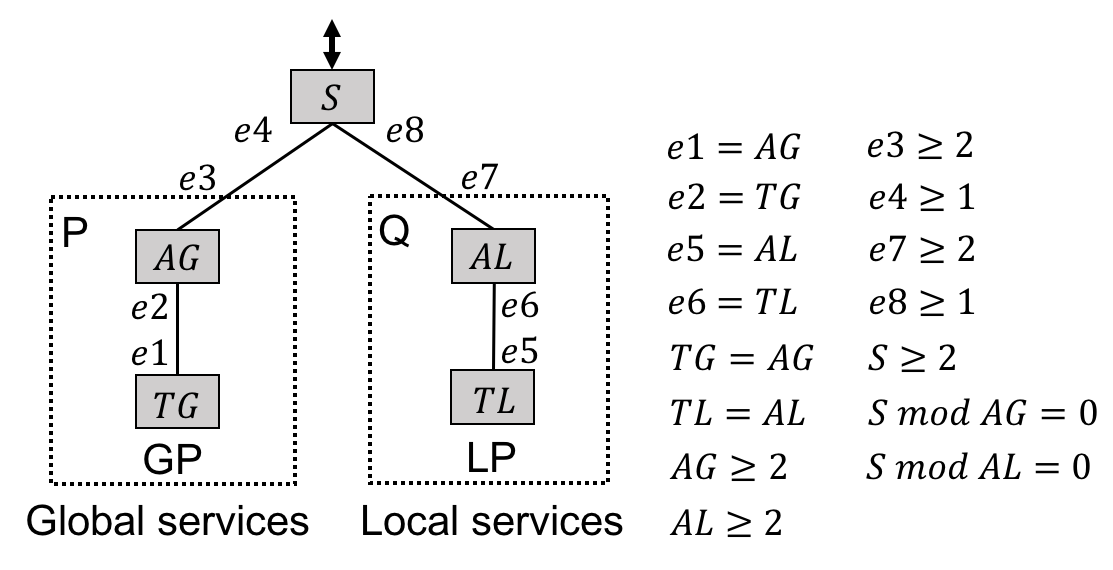
\includegraphics[width=\columnwidth]{figures/example3}
  \caption{Role-based abstraction for the datacenters in Figure~\ref{fig:example}.}
  \label{fig:example3}
  \vspace{-1em}
\end{figure}

In order to refine the abstraction to capture more precisely the kinds of concrete networks of interest,
we introduce a notion of node and edge \emph{multiplicities}. Each edge (and node) is labelled
with a symbolic variable (\EG, $e1, e2, \ldots$) that denotes a constraint on the number of nodes/edges
that may appear in any given concrete network. Operators can then capture concrete network invariants by adding constraints on the symbolic variables using logical formula.

For example, in Figure~\ref{fig:example3}, the first two constraints: $e1 = AG$ and $e2 = TG$ declare that, within any pod P, the number of outgoing edges from $TG$ to $AG$ is equal to the number of nodes that map to $AG$. Similarly, the number of outgoing edges from $AG$ to $TG$ is equal to the number of nodes that map toe $TG$. These constraints capture the fact that, within any given pod, the global aggregators and tors are in a full mesh. Furthermore, the constraints $TG = AG$ and $TG \geq 2$ ensure that the number of concrete nodes in role $TG$ is always equal to the number of concrete nodes in role $AG$. Similar constraints also appear for the local aggregators and tors.
%
The constraint $e3 \geq 2$ says that, in each pod, each aggregator node has at least 2 outgoing edges to nodes in the spine role. Symmetrically, the constraint $e4 \geq 1$ says that, for each pod P, each node in the spine role has at least one outgoing edge to a node in the $AG$ role. Again, similar constraints appear for the local aggregator role. Finally, the constraints $S \geq 2$, $S \pmod AG = 0$, and $S \pmod AL = 0$ ensure that there are at least 2 routers in the spine role, and that the number of spine routers is always divisible by the number of global and local aggregators.
%
The last two constraints are interesting in that they do not involve a simple inequality. In general operators can write constraints using logical formula over any SMT theory. 

All the guarantees provided by \sysname hold for any instantiation of the abstract network. This means that operators can safely expand their network in the future so long as the new network also satisfies these logical constraints.



%Although the concrete \sysname policy can help prevent a number of configuration errors,
%the policy is intricately linked to the actual structure of the concrete network.
%For example, each prefix in the routing constraint is enumerated with its concrete destination
%location, and the definition of the valleyfree constraint depends on the actual routers that
%comprise each tier of the datacenter.
%
%This is unfortunate since any expansion of our datacenter network will require a corresponding
%change to the policy. Furthermore, there is no guarantee that a safe policy can be found
%for the expanded network, and even if one can be found, it may require changes to every
%configuration in the network -- a huge barrier to adoption in practice.

%Abstract \sysname solves this problem in two ways. First, it allows operators to abstract
%the network into a role-based topology and write a routing specification over this abstraction instead.
%Second, it introduces prefix template variables into the language to allow writing policies that are
%parameterized over prefix destination.

\para{Routing Policy}

Now let us configure each of the datacenter networks from \S\ref{sec:motivation} by writing a routing policy over the abstract topology. In \sysname, we can capture the basic routing behavior with the following constraints:
%
\begin{code}
\Define Routing =
    \$PG  \Path \End(TG)
    \$PL  \Path \End(TL)
    \True \Path \Exit(Peer1 \Prefer Peer2)
\end{code}
\noindent%

The first line introduces a prefix \emph{template} variable. It says that traffic for each global prefix associated with the template variable \$PG has the constraint that it should follow a path that ends at its corresponding destination router contained in the abstract TG role. The second line does the same thing for all local prefixes. 
%
The final rule matches all other IP prefix destinations and allows traffic to follow a path that leaves the datacenter through either of its peers (Peer1 or Peer2) with a preference for leaving through Peer1. The \Prefer~ symbol indicates that traffic should satisfy the constraint on the left whenever possible, and only resort to the backup (right) when this is not possible due to failures.%

Next we can capture the constraint that traffic for local prefixes must stay local to the datacenter.
We do this with the following \sysname code:
%
\begin{code}
\Define Locality = 
    \$PL \Path \Always(\In)
\end{code}
\noindent%
%
The Locality constraint applies to any traffic destined for a local prefix described by the \$PL prefix template variable and adds the constraint that the traffic must follow a path that matches an internal location (\IE, a router inside the datacenter) at each hop of the path. This prevents traffic from ever entering from or leaving through an external peer. Finally, we can combine these constraints together as follows:

\begin{code}
Routing & Locality & \Agg(PG, \In -> \Out)
\end{code}
\noindent%

This tells \sysname to find BGP router configurations that satisfy the conjunction of the Routing and Locality constraints. It also declares an additional constraint that we want to perform aggregation for global prefixes by summarizing them as the more general prefix PG at the border of the datacenter (\IE along any edge starting inside our datacenter and ending at a peer outside the datacenter).

When \sysname compiles the above policy, it guarantees that the forwarding behavior of the network will be correct for any concrete instantiation of the abstract network, and for any combination of failures that may occur in the concrete network. Furthermore, \sysname will generate configurations in such a way that, if we want to expand our network, for example by adding additional spine routers as in figure~\ref{fig:example2}, then the expansion can be performed incrementally (\IE, only configurations for routers local to the expansion will need to change).

\subsection{Abstract Analysis}

Although \sysname can ensure correct forwarding behavior independent of the exact concrete topology or failure scenario, it is often useful to be able to ask "what if" questions about other network properties. For example, an operator may require a certain level fault tolerance between between different collections of routers. Importantly, such analysis depends, not only on the network topology, but also on the underlying routing policy. To this end, we develop a sound analysis over abstract topologies to answer questions about the number of disjoint paths between pairs of nodes.

Suppose we want to find a worst-case lower bound on the number of disjoint paths between any global tor and spine router from figure~\ref{fig:example3} after applying the routing policy. This would give us a bound on the fault tolerance for, not only the current datacenter, but any sound expansion of it. Furthermore, this can be used as a lightweight verification tool to detect certain classes of configuration bugs. For example, since we are performing aggregation at the border of the datacenter, we might introduce what is known as an aggregation black hole if enough failures occur to disconnect a tor from a spine.

The disjoint path analysis works in the following way. For each abstract role in the network, we learn invariants about the number of disjoint paths to routers in that role. These invariants contain a sequence of labels followed by a pair of numbers $(i,j)$. For example, the analysis would start with a fact of the form: $S_P S_{TG} (1,1)$. This means that, there is some group of nodes of size 1 in the TG role in some pod P such that each node has 1 disjoint path to it (and all such paths are edge-disjoint). Since we know that the each node in the TG role is in a full mesh with nodes in the AG role within any given pod, we might infer a fact for AG of the form: $S_P A_{AG}(e1,1)$. This says that any group of nodes of size e1 in the AG role is reachable with at least 1 edge-disjoint path to each such node.
%
If we run the abstract analysis over the abstract network from figure~\ref{fig:example3} the analysis will learn a fact of the form $A_{S}(1,2)$, which means that any single spine node is reachable via 2 disjoint paths from any global tor node \ryan{it will actually be 1, we need to add a constraint on e1}. 

Suppose now that we want to disallow paths with valleys (\IE, paths that go down and then up at some point). Such a constraint can be added to the routing policy in \sysname:
\begin{code}
\Define ValleyFree =
    \True \Path \Novalley(\{TL,TG\},\{AL,AG\},\{S\})
\end{code}
\noindent%

This adds a constraint that applies to all traffic and prevents valleys by defining each level in the datacenter.
Because the abstract analysis is policy sensitive, if we were to run the it with the same abstract topology but the new routing policy, it would only be able to infer that there is a single disjoint path to any given spine router in the worst case. In fact this is exactly the case for the concrete network from figure~\ref{fig:example2}.  

%
%The constraint prevents traffic from over taking a path that traverses
%either [Agg->Tor->Agg] or [Spn->Agg->Spn]. The final policy remains the same as before,
%by combining each of these policies together.
%
%


%=====================================================
%
%
%  **Compilation**
%
%
%=====================================================

\section{Configuration Synthesis}
\label{sec:compilation}

Configuration synthesis for network configurations is challenging for a number of reasons. First, although \sysname polices specify stable network-wide routing behavior, actual configurations are per-device and run distributed algorithms to compute routes. Thus the compiler must ensure that the result of the distributed computation matches the policy. Furthermore the distributed computation must compute the correct paths under all possible combinations of failures. Second, \sysname must find configurations that work across any valid concrete network topology matching the abstraction provided as input. Finally, \sysname must ensure that the resulting configurations can be evolved incrementally so that local changes to the topology ensure that only local changes to configurations are required to ensure global routing correctness. 

In this section, we introduce the idea of topology abstraction, describe how \sysname synthesizes network configurations over these abstractions, and formalize the guarantees provided by \sysname.

\subsection{Methane Language}

The syntax introduced in \S\ref{sec:overview} is just syntactic sugar for a core language based on regular expressions. Figure~\ref{fig:syntax} shows a simplified version of the core \sysname syntax that omits some details such as aggregation. The full langauge definition can be found in the appendix. A policy has one or more constraints, each of which consists of a test on the type of traffic being matched and a corresponding set of preferred regular expressions describing network paths. Regular expressions are defined over network locations, where each location is either a router inside the operators network, or an external neighbor. There are two special characters \In~ and \Out, which match any internal and external location respectively. There are two types of predicates: a test for a concrete prefix $d.d.d.d/[d..d]$ matches an IP prefix with value $d.d.d.d$ and length in the range $[d..d]$ where metavariable $d$ represents an integer. For example, the IP prefix 148.0.1.0/[24..32] would match traffic destined for IP address 148.0.1.* with a subnet length between 24 and 32 bits. \ryan{this needs to be explained clearer}.

Converting from the high-level syntax from \S\ref{sec:overview} to the core syntax is straightforward. For example, the predicate $\True$ becomes $0.0.0.0/[0..32]$. Preferences are lifted to the top level of the regular expression when unambiguous. For example, the constraint $\Exit(\sf{Peer1} \Prefer \sf{Peer2})$ becomes $\Exit(\sf{Peer1}) \Prefer \Exit(\sf{Peer2})$ before being rewritten into regular expressions. Each modular set of constraints are joined prefix-by-prefix by taking the intersection of their constraints. For example, the data center policy from \S\ref{sec:overview} would result in the following \sysname policy:
%
\begin{code}
\$PG  \Path \End(TG) & !transit(\Out,\Out),
\$PL  \Path \End(TL) & \Always(\In) & !transit(\Out,\Out),
\True \Path 
    \Exit(Peer1) & !transit(\Out,\Out) \Prefer 
    \Exit(Peer2) & !transit(\Out,\Out)
\end{code}
\noindent%
%
Finally, each constraint desugars to a regular expression. For example, the constraint $\Always(\In)$ becomes $\In^*$ and the constraint $\End({\small \mathsf{T0}})$ becomes $\Sigma^* \cdot \sf{T0}$.

\subsection{Topology Abstraction}

\subsection{Configuration Synthesis}

\subsection{Substitution Theorem}

\begin{easylist}[itemize]
& Define abstractions more formally,
&& e.g., homomorphism between graphs + node/edge constraints

&& First show how to compile to the Product Graph, and from there to the ABGP
&& Show/Define safety analysis simulation relation for both concrete and abstract product graphs
  and how it holds for both.
&& Next define the concretization & subst. functions for translating the abstract policy
   into the concrete policy, using the ABGP example for reference

&& Theorem: if safety analysis holdls in the abstract graph, it holds for the concrete one,
   and the preferences are consistent.

& Give abstraction theorem: commuting of concretization and compilation
\end{easylist}

\begin{figure}[t]\small
  \begin{minipage}[t]{\linewidth}
  \vspace*{-1\baselineskip}
  %
  \[ \begin{array}{rclr}
     pol     &::=& p_1, \dots, p_n & \textit{policies} \\
     p       &::=& t \hspace{.3em} \Path \hspace{.3em} r_1 \Prefer \dots \Prefer r_m & \textit{constraints} \\
     t       &::=& \$x & \textit{template variable} \\
         &\BNFALT& d.d.d.d/[d..d] & \textit{prefix test} \\
     r       &::=& l & \textit{location} \\
         &\BNFALT& \emptyset & \textit{empty set} \\
         &\BNFALT& \In & \textit{internal loc} \\
         &\BNFALT& \Out & \textit{external loc} \\
         &\BNFALT& r_1 \cup r_2 & \textit{union} \\
         &\BNFALT& r_1 \cap r_2 & \textit{intersection} \\
         &\BNFALT& r_1 \cdot r_2 & \textit{concatenation} \\
         &\BNFALT& \NOT r & \textit{path negation} \\
         &\BNFALT& r^* & \textit{iteration} \\
  \end{array} \]%

  \end{minipage}
  \vspace{1em}
  \caption{Simplified \sysname syntax.}
  \label{fig:syntax}
  %\vspace{-1em}
\end{figure}%


\newcommand{\state}[4]{\node[state,#3](#1)[#4]{#2};}
\newcommand{\transition}[4]{\path[->] (#1) edge [#4] node {#3} (#2);}

\begin{figure*}[t!]
  \begin{minipage}[t]{.2\linewidth}
  \hdr{Policy Automata}{}
    \begin{tikzpicture}[>=stealth',shorten >=1pt,auto,node distance=2cm,minimum size=.5cm]
      \state{0}{$0$}{              }{}
      \state{1}{$1$}{right of=0}{accepting}
      \transition{0}{0}{out}{loop above}
      \transition{0}{1}{Peer1}{}
      \transition{1}{1}{in}{loop above}
    \end{tikzpicture}

    \begin{tikzpicture}[>=stealth',shorten >=1pt,auto,node distance=2cm,minimum size=.5cm]
      \state{0}{$0$}{              }{}
      \state{1}{$1$}{right of=0}{accepting}
      \transition{0}{0}{out}{loop above}
      \transition{0}{1}{Peer2}{}
      \transition{1}{1}{in}{loop above}
    \end{tikzpicture}%
  \end{minipage}
  %
  ~~~~~~
  %
  \begin{minipage}[t]{.4\linewidth}
    \hdr{Concrete Topology}{}
    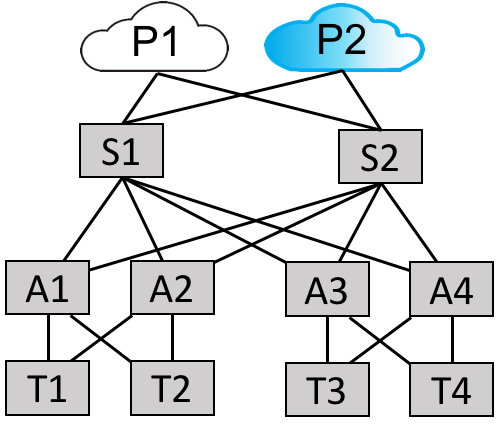
\includegraphics[width=.7\columnwidth]{figures/topology-con}
  \end{minipage}%
  %
  \begin{minipage}[t]{.4\linewidth}
    \hdr{Abstract Topology}{}
    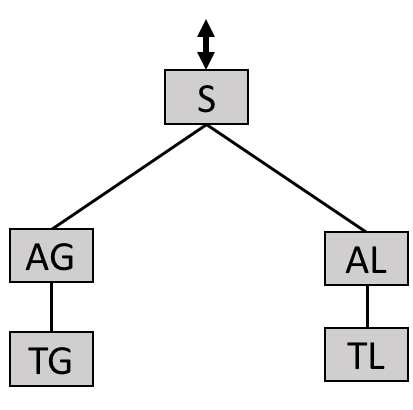
\includegraphics[width=.57\columnwidth]{figures/topology-abs}
  \end{minipage}%

  \vspace{2em}
  \begin{minipage}[t]{.6\linewidth}
    \hdr{Concrete Product Graph}{}
    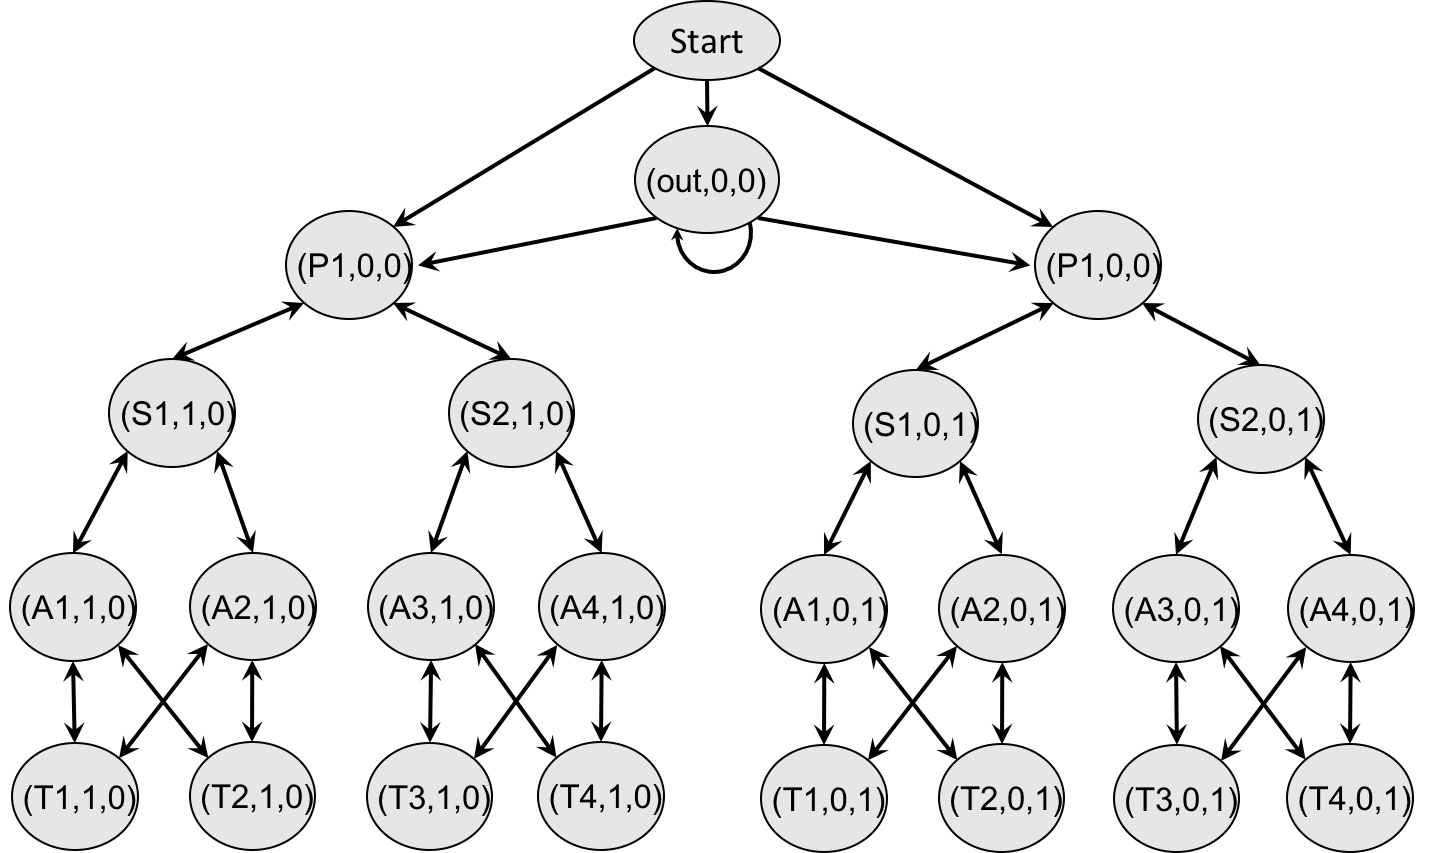
\includegraphics[width=.9\columnwidth]{figures/pg-con}
  \end{minipage}%
  \begin{minipage}[t]{.4\linewidth}
  \hdr{Abstract Product Graph}{}
    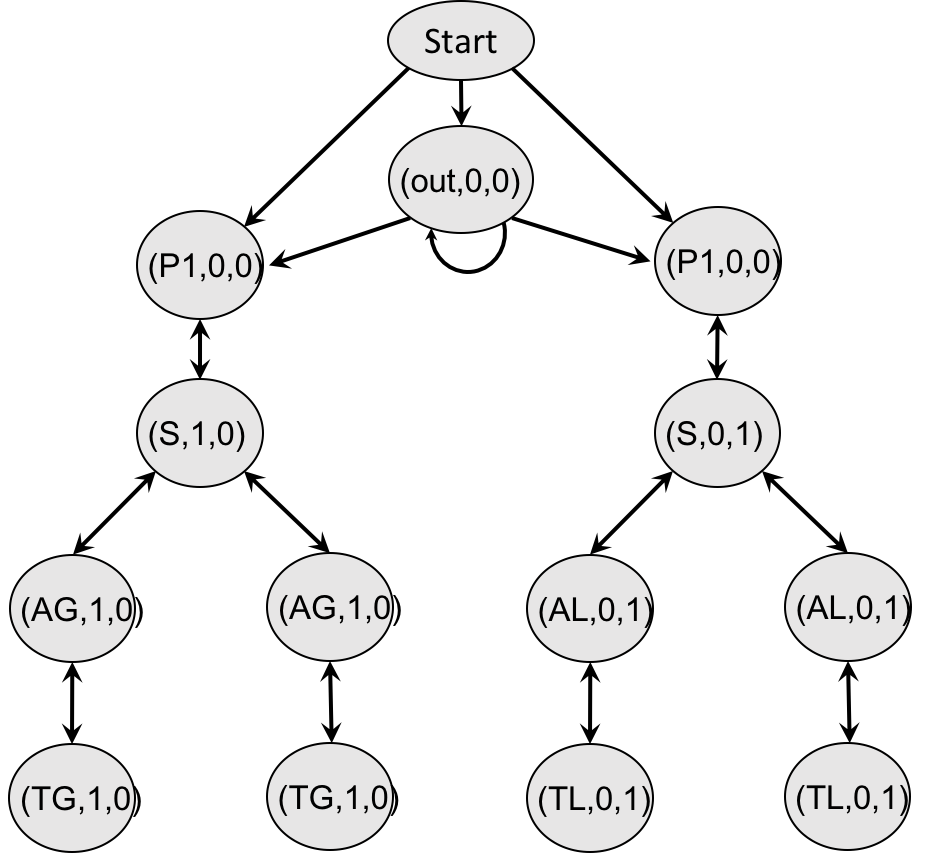
\includegraphics[width=.9\columnwidth]{figures/pg-abs}

  \end{minipage}%

  \hrulefill
  \vspace*{.4em}%

  \caption{Product graph construction for policy $true \Path \Exit(\text{Peer1} \Prefer \text{Peer2})$.}
  \label{fig:example-compilation}
  %\vspace{-1em}
\end{figure*}


%=====================================================
%
%
%  **Abstractions**
%
%
%=====================================================


\section{Analysis}
\label{sec:analysis}


%The examples above use what we call the front end (FE) of \sysname.
%It simplifies operators' task of describing preferred paths, but that simplicity comes at the cost of compilation complexity. The compiler must efficiently compute the sets of paths represented by the intersection of preferences and topology and ensure policy compliance under all failure scenarios.%

%\begin{figure}[t!]
%  \centering
%  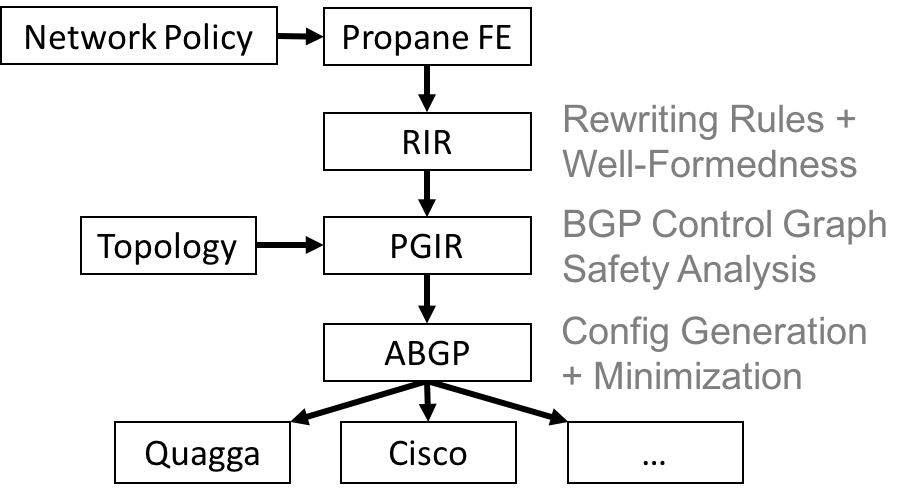
\includegraphics[width=.75\columnwidth]{figures/pipeline}
%  \caption{Compilation pipeline stages for Propane.}
%  \label{fig:pipeline}
%  \vspace{-1em}
%\end{figure}%


%To handle these challenges, we decompose compilation into multiple stages, shown in  Figure~\ref{fig:pipeline}, and develop efficient algorithms for the translation between stages. The first stage of the pipeline involves simple rewriting rules and substitutions from the FE to the core Regular Intermediate Representation (RIR). Policies in RIR are checked well-formedness (\EG, never constraining traffic that does not enter the network), before being combined with the topology to obtain the Product Graph Intermediate Representation (PGIR). The PGIR is a data representation that compactly captures the flow of BGP announcements subject to the policy and topology restrictions. We develop efficient algorithms that operate over the PGIR to ensure policy compliance under failures, avoid BGP instability, and prevent aggregation-induced black holes. Once the compiler determines safety, it translates the PGIR to an abstract BGP (ABGP) representation. ABGP can then be translated into various vendor-specific device
%configurations as needed.


%The \sysname FE is just a thin layer atop the RIR for describing preference-based path constraints.
%Figure~\ref{fig:rir-syntax} shows the RIR syntax. A policy has one or more constraints. The first kind of constraint is a test on the type of route and a corresponding set of preferred regular paths. Regular paths are regular expressions where the base characters are abstract locations representing either a router or an external AS. Special \In{} and \Out{} symbols refer to any internal or external location respectively. In addition, $\Sigma$ refers to any location. We also use the standard regular expression abbreviation $r^+$ for $r \cdot r^*$, a sequence of one or more occurrences of $r$. Predicates ($t$) consist of logical boolean connectives (and, or, not) as well as tests that match a particular prefix (or group of prefixes) and tests for route advertisements with a particular community value attached (\IE, an integer value associated with a path).%
%

%\sysname also supports constraints on the control-plane behavior of BGP. For example, prefix aggregation is an important optimization to reduce routing table size. A constraint of the form $agg(x,ln)$ tells the compiler to perform aggregation for prefix $x$ across all links described by $ln$. It is also often useful to be able to add community tags to exported routes in BGP (\EG, to communicate non-standard information to peers). A constraint of the form $tag(d,t,ln)$ adds community tag $d$ for any prefixes matching $t$ across links $ln$.
%%
%We list only the route aggregation and community tagging constraints in Figure~\ref{fig:rir-syntax}, but \sysname also supports other constraints such as limiting the maximum number of routes allowed between ASes, or enabling BGP multipath.


%\para{Semantics}

%We give a semantics to RIR programs using sets of ranked paths. Each path constraint $r_1 \Prefer \dots \Prefer r_j$ denotes a set of ranked network paths. A network path is a topologically valid string of abstract locations $l_1 l_2 \dots l_k$. We use the notation $\abs{p}$ to denote the length of the path $p$. A regular expression $r$ matches path $p$, if $p \in \mathcal{L}(r)$, that is, the path is in the language of the regular expression. Paths are ranked lexicographically according to (1) the most preferred regular expression matched, and (2) as a tie breaker, the path length. Lower ranks indicate \emph{more} preferred paths. More formally, a path $p$ has rank:
%$$(\min_i \set{ p \in \mathcal{L}(r_i) }, \abs{p})$$
%%
%The set of ranked paths depends on which paths are valid in the topology, and thus when failures occur, the most preferred routes change.
%%
%For any source $s$ and destination $d$, \sysname will send traffic along the highest ranked available path from $s$ to $d$.


%\para{From FE to RIR}

%The first stage in \sysname compilation reduces the FE to the simpler RIR from Figure~\ref{fig:rir-syntax}.
%The main differences between the FE and RIR are: $i)$ FE allows the programmer to specify constraints using a series of (modular) definitions, and combine them later, $ii)$ FE provides high-level names that abstract sets of routes and groups of prefixes/neighbors, and $iii)$ FE allows the preference operator to be used more flexibly.%

%A key constraint when translating FE to RIR is ensuring that all specified routes are well-formed. In particular, each regular path constraint $r$ must satisfy $r \subseteq \Out^* \cdot \In^+ \cdot \Out^*$. It ensures that users only control traffic that goes through their network at some point, and that such traffic does not loop back multiple times through their network.%

%The translation from FE to RIR is based on a set of rewriting rules.
%The first step merges separate constraints. It takes the cross product of per-prefix constraints, where logical conjunction ($r_1 ~\AND~ r_2$) is replaced by intersection on regular constraints ($r_1 \Intersect r_2$), logical disjunction is replaced by union, and logical negation ($\NOT r$) is replaced by path negation ($\Any \cap \NOT(r)$). The additional constraint $\Any$ ensures the routes are well-formed by restricting the paths to only those that go through the user's network.
%%
%For example, in the datacenter FE configuration from \S\ref{sec:propane}, combining the \CD{Locality} and \CD{Ownership} policies results in the following RIR:%

%\begin{code}
%PG1 \Path \End(A)
%PG2 \Path \End(B)
%PL1 \Path \textbf{only}(\In) \Intersect \End(E)
%PL2 \Path \textbf{only}(\In) \Intersect \End(F)
%\True \Path \Exit(\Out)
%\end{code}%

%The next step rewrites the high-level constraints such as $\Exit$ according to the equivalences in Figure~\ref{fig:rir-syntax}. Since preferences can only occur at the outermost level for an RIR expression, the final step is to ``lift" occurrences of the preference operator in each regular expression. For example, the regular expression $r \cdot (s ~\Prefer~ t) \cdot u$ is lifted to $(r \cdot s \cdot u) \Prefer (r \cdot t \cdot u)$ by distributing the preference over the sequence operator. In general, we employ the following distributivity equivalences:
%%
%\[
%\begin{array}{c}
%  r \odot (s_1 \Prefer \dots \Prefer s_n) = (r \odot s_1) \Prefer \dots \Prefer (r \odot s_n) \\
%  (s_1 \Prefer \dots \Prefer s_n) \odot r = (s_1 \odot r) \Prefer \dots \Prefer (s_n \odot r)
%\end{array}
%\]
%%
%where $\odot$ stands for an arbitrary regular binary operator, and $r$ is a policy with a single preference.
%%
%In cases where $r$ does not contain a single preference, such as $(s ~\Prefer~ t) \cdot (u ~\Prefer~ v)$, it is not clear which of the paths $s \cdot v$ or $t \cdot u$ is preferred. \sysname rejects such ambiguous policies, requiring instead that operators explicitly specify which paths to prefer --- for example as $(s \cdot u) ~\Prefer~ (s \cdot v) ~\Prefer~ (t \cdot u) ~\Prefer~ (t \cdot v)$.
%%
%Policies that contain preferences nested under a unary operator (\IE, \textit{star} or \textit{negation}) are also rejected by \sysname as invalid.




%\subsection{Product graph IR}

%Now that the user policy exists in a simplified form, we must consider the topology. In particular, we want a compact representation that describes all the possible ways BGP route announcements can flow through the network subject to the policy and topology constraints. The PGIR captures these constraints by ``intersecting" each of the regular automata corresponding to the RIR path preferences with the topology. Paths through the PGIR correspond to real paths through the topology that satisfy the user constraints.



%\para{Formal definition}

%While paths in an RIR policy describe the direction traffic flows through the network, to implement the policy with BGP we are concerned about the way control-plane information is disseminated --- route announcements flowing in the opposite direction. To capture this idea, for each regular expression $r_i$ in an RIR policy, we construct a deterministic finite state machine for the reversed regular expression. An automata for regular expression $r_i$ is defined as a tuple ($\Sigma, Q_i, F_i, q_{0_i}, \sigma_i$). The alphabet $\Sigma$ consists of all abstract locations (\IE, routers or ASes), $Q_i$ is the set of states for automaton i, $F_i$ is the set of final states, $q_{0_i}$ is the initial state, and $\sigma_i \colon Q_i \times \Sigma \rightarrow Q_i$ is the state transition function.
%%
%The topology is represented as a graph ($V, E$), which consists of a set of vertices $V$ and a set of directed edges $E \colon V \times V$.
%%
%The combined PGIR is a tuple ($V'$, $E'$, $s$, $e$, $P$) with
%vertices $V' \colon V \times Q_1 \times \dots \times Q_j$,
%edges $E' \colon V' \times V'$,
%a unique starting vertex $s$,
%a unique ending vertex $e$,
%and a preference function $P \colon V' \rightarrow 2^{\set{1, \dots, j}}$ , which maps nodes in the product graph to a set of path ranks.%

%For a PGIR vertex $n = (l, \dots) \in V'$, we say that $n$ is a \emph{shadow} of topology location $l$. We also write $\tilde{n} = l$ to indicate that the topology location for node $n$ is $l$. When two PGIR nodes $m$ and $n$ shadow the same topology location (\IE, $\tilde{m} = \tilde{n}$), we write $m \approx n$.%

%Throughout the remainder of the paper, we will use the convention that metavariables $m$ and $n$ stand for PGIR nodes and $l$ stands for a topology location. Capital letters like $X$ refer to concrete topology locations, while capital letters with subscripts such as $X_1$ and $X_2$ refer to concrete PGIR nodes that share a topology location (\IE, $\tilde{X_1}$ = $\tilde{X_2} = X$).

%\para{From RIR To PGIR}

%Let $a_i$ and $b_i$ denote states in the regular policy automata.
%The PGIR is constructed by adding an edge from $m = (l_m, a_1, \dots, a_k)$ to $n = (l_n, b_1, \dots, b_k)$ whenever $\sigma_i(a_i, l_n) = b_i$ for each $i$ and $(l_m,l_n) \in E$ is a valid topology link.
%%
%Additionally, we add edges from the start node $s$ to any $n = (l, a_1, \dots, a_k)$ when $\sigma_i(q_{0_i}, l) = a_i$ for each $i$.
%%
%The preference function $P$ is defined as $P(n) = \set{i~\vert~a_i \in F_i} $. That is, it records the path rank of each automaton that has reached a final state.
%%
%Finally, there is an edge from each node in the PGIR such that $P(n) \neq \emptyset$ to the special end node $e$. We write $(m \leq_{rank} n)$ if either $P(m) = P(n) = \emptyset$ or $min ~ P(m) \leq min ~ P(n)$, which means that paths ending at PGIR node $m$ are better (lower rank) than paths ending at $n$.%
%

%Intuitively, the PGIR tracks the policy states of each automaton as route announcements move between locations.
%%
%Consider the topology in Figure~\ref{fig:example-compilation}. Suppose we want a primary route from neighbor W that allows traffic to enter the network at $A$ and utilize the C--D link before leaving the network (through $X$ or $Y$). As a backup, we also want to allow traffic to enter the network from $B$, in which case the traffic can also utilize the C--E link before leaving the network. For simplicity, we assume that the route ends in either $X$, $Y$, or $Z$. The RIR for the policy could be written as:
%%
%$$(\CD{W} \cdot \CD{A} \cdot \CD{C} \cdot \CD{D} \cdot \Out) \Prefer (\CD{W} \cdot \CD{B} \cdot \In^+ \cdot \Out)$$
%%
%Figure~\ref{fig:example-compilation} shows the policy automata for each regular expression preference. Since we are interested in the flow of control messages, the automata match backwards.
%%
%The figure also shows the PGIR after intersecting the topology and policy automata. Every path in the PGIR corresponds to a concrete path in the topology. In particular, every path through the PGIR that ends at a node $n$ such that the preference function $P(n) = \set{i_1, \dots, i_k}$ is non-empty, is a valid topological path that satisfies the policy constraints and results in a particular path with preferences $i_1$ through $i_k$.
%%
%For example, the path $X \cdot D \cdot C \cdot A \cdot W$ is a valid path in the topology that BGP route announcements might take, which would lead to obtaining a path with the lowest (best) rank of $1$.
%BGP control messages can start from peer X, which would match the $\Out$ transition from both automata, leading to state $1$ in the first automaton, and state $1$ in the second automaton. This possibility is reflected in the product graph by the node with state $(X,1,1)$. From here, if X were to advertise this route to D, it would result in the path $D \cdot X$, which would lead to state $2$ in the first automaton, and state $2$ in the second automaton, and so on.
%%
%The ``--" state indicates the corresponding automaton cannot accept the current path or any extension of it. Since
%node $(W,5,-)$ is in an accepting state for the first automaton, it indicates that this path has rank 1.



%\subsection{Failure-safety analysis}

%To implement path preferences in routing, BGP uses local preferences on a per-device basis. However, the distributed nature of BGP makes setting preferences locally to achieve a network-wide routing policy difficult. This task becomes even more challenging in the presence of failures since routers running BGP lack a global view of the network.

%\para{An illustrative example}

%To demonstrate the difficulty of generating device-local preferences, consider the simple policy for the topology in Figure~\ref{fig:unimplementable}, which says to prefer the top path over the bottom path:
%%
%$(\CD{A} \cdot \CD{B} \cdot \CD{D} \cdot \CD{E} \cdot \CD{G})  \Prefer (\CD{A} \cdot \CD{C} \cdot \CD{D} \cdot \CD{F} \cdot \CD{G})$.
%%
%How could such a policy be implemented in BGP? Suppose we set the local preferences to have $D$ prefer $E$ over $F$, and have $A$ prefer $B$ over $C$. This works as expected under normal conditions, however, if the A--B link fails, then suddenly $D$ has made the wrong decision by preferring $E$. Traffic will now follow the
%$A \cdot C \cdot D \cdot E \cdot G$ path, even though this path was not allowed by the policy. Thus, the distributed implementation has used a route that is not allowed by the policy. To make matters worse, the second preference for the path $A \cdot C \cdot D \cdot F \cdot G$ is available in the network but not being used. Thus, a path for the best possible route available after the A--B failure exists in the network, but the distributed implementation will not find it.
%%
%The first problem could be fixed by tagging and filtering route advertisements appropriately so that $C$ rejects routes that go through $E$, however the second problem cannot be fixed. In fact, this policy cannot be implemented in BGP in a way that is policy compliant under all failures since $D$ cannot safely choose between $E$ and $F$ without knowing whether the A--B link is available.


%\para{Problem formulation}

%The problem of determining local preferences for each router is reflected in the structure of the PGIR. Whenever a given router appears as multiple shadow nodes in the PGIR, the compiler must decide which shadow to prefer.
%%
%In the example from Figure~\ref{fig:example-compilation}, the topology node $C$ can receive an advertisement from $E$ in shadow $(C,-,2)$ or from $D$ in shadow $(C,3,2)$.
%%
%%
%The compiler must determine a \emph{total ordering} of shadow nodes for each router, which reflects the relative preference of advertisements received in each shadow and should be consistent with path ranks.
%%
%For example, if $C$'s shadow $(C,3,2)$ can be preferred to $(C,-,2)$, written as $(C,3,2) \leq_{lp} (C,-,2)$, $C$ can prefer advertisements from $(D,2,2)$ over $(E,-,2)$. $D$ and $E$ tag their advertisements to let $C$ know which shadow sent the advertisement. Section \ref{sec:abgp} discusses tagging in detail.

%\begin{figure}[t!]
%  \centering
%  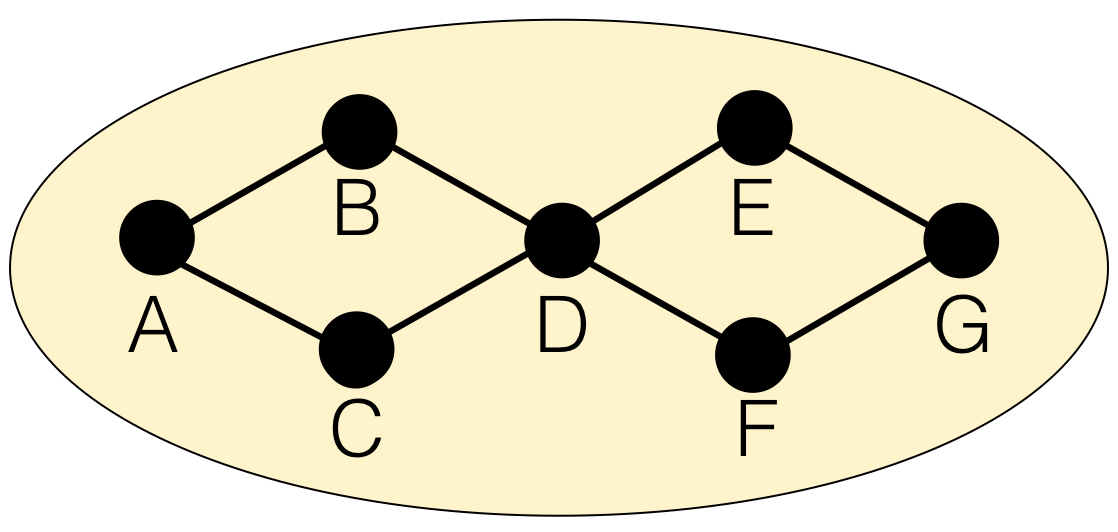
\includegraphics[width=.5\columnwidth]{figures/unimplementable}
%  \caption{A network where the policy $(\CD{A} \cdot \CD{B} \cdot \CD{D} \cdot \CD{E} \cdot \CD{G}) \Prefer (\CD{A} \cdot \CD{C} \cdot \CD{D} \cdot \CD{F} \cdot \CD{G})$ is unimplementable in BGP under arbitrary failures.}
%  \label{fig:unimplementable}
%  %\vspace{-1em}
%\end{figure}



%\para{Regret-free preferences}

%To order PGIR shadows ($\leq_{lp}$) for each router in a way that is policy-compliant under all failures, we introduce the notion of \emph{regret-free} preferences, motivated by the observations from the example in Figure~\ref{fig:unimplementable}. A router (location) $l$ has a regret-free preference for a set of advertisements $A$ over $B$ if, whenever $l$ selects an advertisement to destination $d$ from $A$ over another from $B$, there is always some policy-compliant path to $d$ that is at least as good ($\leq_{rank}$ for the final node along the path) as any possible path (not necessarily from $l$) to $d$ if $l$ had selected an advertisement from $B$ instead. In other words, the preference of $A$ over $B$ at $l$ is regret-free if $l$ is never (under any failure) worse-off by choosing an advertisement from $A$ when available. The notion of regret-free preferences can be lifted to PGIR nodes by considering the set of advertisements available to each node.%

%In the example of Figure~\ref{fig:example-compilation}, the choice for $C$ to prefer shadow $(C,3,2)$ to $(C,-,2)$ is regret-free, since there will always be at least as good a path to destination $W$ regardless of any failures that might occur in the network. For example, if the $C$--$A$ link fails, then there is still a backup path from $(C,3,2)$ to $(W,-,4)$ that is just as good as any path from $(C,-,2)$. Likewise, any combination of failures to disconnect $(C,3,2)$ from $(W,-,4)$ would also disconnect $(C,-,2)$ from $(W,-,4)$.


%\para{A preference inference algorithm}


%Searching for precise regret-free preferences in general is hard, and clearly enumerating all possible combinations of failures and preference orderings is intractable. We thus adopt a conservative analysis that we found to be effective and efficient in practice. The idea is to $i)$ search for regret-free preferences by comparing the set of paths available after accepting advertisements in two different PGIR shadows $N_1$ and $N_2$ of topology node $N$, and $ii)$ refine the comparison when necessary by considering where the announcements must have traversed before arriving at $N_1$ or $N_2$.

%\begin{algorithm}[t!]
%\caption{Inferring regret-free preferences}
%\label{alg:failures}
%\begin{algorithmic}[1]
%\Procedure{Regret-free($G$, $N_1$, $N_2$)}{}
%  \If {$N_1 \not\approx N_2$} \Return false
%  \EndIf
%  \State $q \gets Queue()$
%  \State $q.Enqueue (N_1, N_2)$
%  \While {$!q.Empty()$}
%    \State $(m,n) \gets q.Dequeue()$
%    \If {$m \nleq_{rank} n$}
%      \Return false
%    \EndIf
%    \For {$n'$ in adj($G$, $n$)}
%      \If {\big($\exists m' \in \textup{adj}(G,m), m' \approx n'$\big)}
%        \If {$(m',n')$ not marked}
%          \State {mark $(m',n')$ as seen}
%          \State $q.Enqueue(m',n')$
%        \EndIf
%      \Else { \Return $false$}
%      \EndIf
%    \EndFor
%  \EndWhile \\
%  \hspace{\algorithmicindent} \Return true
%\EndProcedure
%\end{algorithmic}
%\end{algorithm}


%Algorithm~\ref{alg:failures} checks whether one shadow can be preferred to another ($N_1 \leq_{lp} N_2$). It walks from nodes $N_1$ and $N_2$ and ensures that for every \textit{step} $N_2$ can take to some new topology location, $N_1$ can, at the very least, also take a step to an equivalent topology location $(\approx)$. When there is no such equivalent step, the algorithm attempts to take into account where the advertisement must have already traversed. In particular, it checks if there is an equivalent dominator node and, if so, walks from this new node instead.
%%
%The idea is that, since the advertisement must have already passed through the dominator, we can check to see if we are guaranteed to find paths that are at least as good from this new node instead.
%%
%At each step, it requires that the current node reachable from $N_1$ has a path rank that is at least as good as that of the current node reachable from $N_2$ ($m \leq_{rank} n$). The intuition here is that if $m \nleq_{rank} n$, then we can very likely fail every edge in the topology except for the path that leads to the current $m$ and $n$, thereby generating a counterexample.
%Algorithm~\ref{alg:failures} terminates since the number of related states $(m,n)$ that can be explored is finite.%

%For each router in the topology, local preferences are now obtained by sorting the corresponding PGIR shadows according to the $(\leq_{lp})$ relation determined by Algorithm~\ref{alg:failures}. If two nodes are incomparable, then the compiler rejects the policy as unimplementable.



%\para{Avoiding loops}

%The checks for failure safety described above overlook one critical point: A better (lower rank) path might not be available due to loops rejected by BGP.%

%Consider the partial product graph shown in Figure~\ref{fig:avoiding-loops}. Our preference inference algorithm will determine that node $X_1$ should be locally preferred to node $X_2$ since this will result in a better (lower ranked) path to destination $A$. However, when applying Algorithm~\ref{alg:failures}, we failed to take into account the possibility of loops. In particular, node $A_2$ may be unusable for advertisements that go through $X_1$ since the advertisement may have already gone through $A_1$ previously. In this case, $X$ will have made the wrong choice since preferring $X_2$ would have resulted in a better path for the destination $A$ (a path of rank 3 instead of 4).%

%On the other hand, this would not have been a problem if paths ending at $A_1$ had a lower rank than those ending at $A_2$ or $A_3$. For example, if paths ending at $A_1$ had rank 1, then any time $A_2$ is unusable due to a loop with $A_1$, it ultimately does not matter since $A_1$ is preferred anyway.
%%
%In fact, checking if we are never worse off using $A_1$ instead of $A_2$ corresponds exactly with determining if $A$ has a regret-free preference for $A_1$ over $A_2$.
%%
%More specifically, the compiler checks that, any time there are two shadows $N_1$ and $N_2$ for the same topology location, where $N_1$ appears ``above'' (\IE, can reach) $N_2$ in the PGIR, then $N_1$ must be strictly preferred to $N_2$ (\IE, $N_1 <_{lp} N_2$).

\subsection{Other properties}
\label{sec:property-checking}

\begin{easylist}[itemize]
& Graph homomorphism is not enough -- to coarse an overapproximation
&& Use node/edge multiplicites to capture more precise constraints on concrete topologies
&& Show a bunch of examples of fattree, bcube, dcell, hyperX, facebook, google, F10, etc.
& K-disjoint path analysis
&& Useful for aggregation safety (black holes) & reachability
&& Inference rules as an abstract interpretation using Z3
\end{easylist}

\newcommand{\inference}[4]{
    \node[draw, anchor=west] at (#1 + .4, 1.25) {#3};
    \node at (#1 + .34, .6) {$e_1$};
    \node at (#1 + .34, 1.9) {$e_2$};
    \node at (#1, -.8) {#2};
    \node at (#1, 3.3) {#4};
    \draw [] (#1, 2.5) circle [radius=0.45] node {$m$};
    \draw [] (#1, 0) circle [radius=0.45] node {$n$};
    \draw [] (#1, .45) -- (#1, 2.05);
}

\begin{figure*}[t!]
  \begin{minipage}[t]{.5\linewidth}%
  \begin{tikzpicture}
    \inference{0}{L$(j,k)$}{$\vDash e_1 > 0$}{S$(min(j*k,e_1),1)$}
    \inference{5}{A$(j,k)$}{$e_2 > 0$}{A$(1,min(j,e2))$}
    \inference{10}{L$(j,k)$}{$e_1=n$}{A$(min(j*k,n),1)$}
    \inference{15}{L$(j,k)$}{$e_1=n$}{A$(1,j)$}
  \end{tikzpicture}
  \end{minipage}

  %
  \vspace*{3em}
  %
  \begin{minipage}[t]{.5\linewidth}%
  \begin{tikzpicture}
    \inference{0}{L$(j,k)$}{$e_1 > 0$, $e_2 > 0$}{S$(min(j*k,n-\dfrac{(m-j)*e_1}{e_2}),1)$}
    \inference{10}{L$(j,k)$ ~~~ L$(j- m ~\text{mod}~ \big(\dfrac{n}{e_1}\big),1)$}{$e_1 > 0$, $e_2 > 0$}{}
  \end{tikzpicture}
  \end{minipage}

  \vspace*{1em}
  \hrule
  \vspace*{1em}
  \caption{Abstract k-disjoint path analysis inference rules.}
  \label{fig:abstract-analysis}
  %\vspace{-1em}
\end{figure*}




%\subsection{Aggregation-safety analysis}
%\label{sec:agg-safety}

%As shown in \S\ref{sec:motivation}, aggregation can lead to subtle black-holing of traffic when failures occur. Determining when this can happen requires knowledge, not only of the topology, but also of the policy. For instance, a policy might require that all traffic for a particular prefix go over a single link before being aggregated. If that one link fails, a black hole might be introduced.
%%
%Because the PGIR encodes the complete user policy and topology, \sysname can efficiently check that aggregates do not black hole traffic for up to $k$ failures.%

%We view the aggregation problem as a variant of the min-cut problem in the PGIR. Specifically, for each prefix that falls under an aggregate, we are interested in finding a lower bound on the number of failures required to disconnect the prefix's origin from its aggregation point. The difficulty, however, is that each link in the topology might appear as multiple links in the PGIR, thus preventing the direct application of standard min-cut algorithms.
%%%

%Instead, we adopt the following simple strategy: $i)$ pick a random path in the PGIR between the prefix's origin and aggregation point, $ii)$ remove all similar edges in the PGIR for each topology edge along the chosen path, and $iii)$ repeat until no such path exists.
%Because each path chosen is both policy compliant and edge disjoint (due to ii), the number of paths that we are able to remove lower bounds the number of failures required to disconnect the prefix from its aggregate, subject to the policy constraints.%
%

%Recall the datacenter example from \S\ref{sec:motivation}, with the policy
%\CD{PG1} \Path \text{ }\End(\CD{A}), where \CD{PG1} falls under the \CD{PG} aggregate. Figure~\ref{fig:aggregation-safety} shows the PGIR for \CD{PG1}. Since we know aggregation will occur at $X$, and that the \CD{PG1} prefix will originate at $A$, we can compute the number of failures it would take to disconnect $A$ from $X$. We could remove the $A$--$D$--$X$ path first and would then need to remove any other $A$--$D$ or $D$--$X$ links from the PGIR (in this case none). Next, we could remove the links along the $A$--$C$--$X$ path, repeating the process. Because $A$ is now disconnected from $X$, 2 is a lower bound on the number of failures required to introduce an aggregation black hole for prefix \CD{PG1}. This process is repeated for other aggregation locations (\EG, $Y$).


%\subsection{Abstract BGP}
%\label{sec:abgp}
%The final stage of our compiler translates policies from PGIR to a vendor-neutral abstraction of BGP (ABGP).

%\para{From PGIR to ABGP}

%\newcommand{\highlight}[1]{%
%  \colorbox{red!50}{$\displaystyle#1$}}
%\newcommand{\Router}[1]{\KW{Router} #1:}
%\newcommand{\REGEX}[1]{\texttt{regex}(#1)}
%\newcommand{\PEER}{\texttt{peer}}
%\newcommand{\COMM}{\texttt{comm}}
%\newcommand{\MED}{\texttt{MED}}
%\newcommand{\Arrow}{\ensuremath{\leftarrow}}%

%\begin{figure}[t!]
%\begin{code}
%  \Router{A}
%    Match \PEER=C, \COMM=(3,2)
%      Export \COMM \Arrow (4,2),
%             \MED \Arrow 80, \PEER \Arrow W
%  \Router{B}
%    Match \PEER = C, \COMM = (-,2) or (3,2)
%      Export \COMM \Arrow (-,3), \COMM \Arrow \text{noexport},
%             \MED \Arrow 81, \PEER \Arrow W
%  \Router{C}
%    Match[LP=99] \PEER = E, \COMM = (-,2)
%      Export \COMM \Arrow (-,2), \PEER \Arrow B
%    Match \PEER = D, \COMM = (2,2)
%      Export \COMM \Arrow (3,2), \PEER \Arrow A,B
%  \Router{D}
%    Match \REGEX{X + Y}
%      Export \COMM \Arrow (2,2), \PEER \Arrow C
%  \Router{E}
%    Match \REGEX{Z}
%      Export \COMM \Arrow (-,2), \PEER \Arrow C
%  \end{code}
%  \vspace{-2em}
%  \caption{Abstract BGP router configurations. \label{fig:abgp-config}}
%  \vspace{-1em}
%\end{figure}



%=====================================================
%
%
%  **Implementation**
%
%
%=====================================================


\section{Implementation}
\label{sec:implementation}

The \sysname compiler is implemented in approximately 9500 lines of F\# code. The compiler accepts both concrete and abstract topologies and will generate router configurations for open-source Quagga routers. Operators can specify their required fault tolerance level for aggregation safety. The abstract safety analysis uses Z3Opt \ryan{reference} to minimize variables subject to the annotated constraints. Since the analysis typically calls Z3 with many times with relatively simple optimization problems, we use a timeout of 200ms. 

The compiler performs the following to improve its performance.

\para{Z3 memoization}

Although the k-disjoint path analysis takes place over the Product Graph representation, which may differ from the topology (e.g., for non-shortest paths routing), each application of the inference rules from figure~\ref{fig:abstract-analysis} depends only on the topology. Therefore, we lazily apply the rules and cache the satisfiability and minimization calls to Z3 after their first use. Doing this significantly speeds up the failure safety analysis. Furthermore, the cached results can be shared across different prefixes, each of which may have a unique Product graph representation. In practice, this means that after performing the abstract analysis for one prefix, the analysis becomes essentially "free" for any subsequent prefixes.

\para{Fast Substitution}

Substitution after compiling a policy abstractly can be expensive since each router must substitute all template variables for each of its connected peers. In practice, because many routers often share the same concrete peers, memoizing the substitution function greatly improves performance.


%=====================================================
%
%
%  **Evaluation**
%
%
%=====================================================


\section{Evaluation}
\label{sec:evaluation}

We apply \sysname on policies for backbone and datacenter networks. We aim to evaluate the expressiveness of our abstract multiplicity annotations, the precision of the abstract disjoint-path analysis, and the compilation time of \sysname both with abstraction and without.

\subsection{Analysis precision}

\begin{figure}[t!]
  \begin{center}
      \begin{tabular}{| l | c | c | c |}
      \hline
      \textbf{Topology} & \textbf{Fixed} & \textbf{Reachable} & \textbf{K-paths} \\ \hline
      Google Fattree & & \cmark & \cmark  \\ \hline
      Facebook Fattree & & \cmark & \cmark \\ \hline
      Microsoft Fattree & & & \\ \hline
      F10 Fattree & & \cmark & \cmark \\ \hline
      BCube & $k$ & \cmark & \xmark \\ \hline
      DCell & $k$ & \cmark & \xmark \\ \hline
         %& HCN & $h$ & \cmark & \xmark \\
      Butterfly & $n$ & \cmark & \cmark \\ \hline
      Hypercube & $N$ & \cmark & \cmark \\ \hline
      HyperX & $L$ & \cmark & \cmark \\ \hline
      \end{tabular}
  \end{center}
  \caption{Abstract Analysis Precision.}
  \label{fig:analysis-precision}
\end{figure}

%\begin{figure}[t!]
%  \begin{center}
%      \begin{tabular}{| l l | c | c | c |}
%      \hline
%      \textbf{Topology} & \textbf{Variant} & \textbf{Fixed} & \textbf{Reachable} & \textbf{K-paths} \\ \hline
%      Fattree
%         & Google &  & \cmark & \cmark  \\
%         & Facebook &  & \cmark & \cmark \\
%         & F10 &  & \cmark & \cmark \\ \hline
%      Recursive
%         & BCube & $k$ & \cmark & \xmark \\
%         & DCell & $k$ & \cmark & \xmark \\ \hline
%         %& HCN & $h$ & \cmark & \xmark \\
%      Hypercube
%         & Standard & $N$ & \cmark & \cmark \\
%         & HyperX & $L$ & \cmark & \cmark \\ \hline
%      Random \footnote{foo}
%         & Scafida &  & ??? & ??? \\
%         & JellyFish &  & ??? & ??? \\
%      \hline
%      \end{tabular}
%  \end{center}
%  \caption{Abstract Analysis Precision.}
%  \label{fig:analysis-precision}
%\end{figure}

We evaluate the expressiveness and precision of our abstract analysis on a range of different network topologies found in both the network literature and production. For each topology in figure~\ref{fig:analysis-precision} we define a suitable abstraction. Since many topologies have tunable parameters (e.g., the recursion depth $k$ for the DCell topology), we list all such parameters that are fixed for our abstraction. We implement a shortest path routing policy over the topology and record the precision of the abstract analysis in terms of whether or not it is able to accurately prove reachability and/or the correct number of disjoint paths between all pairs of nodes.

\para{Fat Tree Topologies}

The Fat Tree topology is one of the most widely used datacenter topologies. We look at the precision of our analysis on three variants of the Fat Tree~\cite{foo} topology used in practice: the Google Fat Tree, the Facebook Fat Tree, and the F10 fault tolerant Fat Tree. For each Fat Tree variant, we use a tiered abstraction similar to that in our previous example \ryan{Reference}. Each Fat Tree topology is parameterized over the number of pods $k$, which can be scaled up in the abstraction to allow for expansion. For all Fat Tree variants, the analysis is precise enough to determine the exact number of disjoint paths between all pairs of concrete routers.

\para{Recursive Topologies}

We also model several recursive topologies using our abstractions. These include the BCube and DCell topologies. Each topology includes a recursion depth parameter ($k$), which we must fix. For a recursive topology with depth $d$, we model it as an abstract topology consisting of abstract nodes for each of the depth $d-1$ subcomponents. This allows for safe expansion within a subcomponent, but not from increasing the recursion depth. The analysis is able to accurately determine reachability (i.e., at least 1 disjoint path) for each recursive topology, but is overly conservative in determining k-disjoint paths. For the BCube topology, it is able to to determine the correct number of disjoint paths between some pairs of nodes, but not all.

\para{Hypercube Topologies}

Hypercube variants can be used as an alternative to Clos-style topologies for networks with high-radix (port density) switches. The HyperX topology can be viewed as a generalization of the hypercube, which includes parameters $L$ for the lattice dimension of the network, $S_i$ for the node multiplicity of each dimension $i$, $K_i$ for the bandwidth of links for each dimension, and $T$ for the number of terminal nodes (servers) connected to each router. For a fixed number of dimensions $L$, we abstract each full mesh of $S_L$ nodes into its own abstract node. The $S_{x-1}$ groups of abstract nodes can be captured using pods of the abstract $S_x$ nodes.

%\para{Random Network Topologies}
%
%Random networks such as Scafida and Jellyfish have seen a great deal of interest in academia. These topologies were designed with an eye towards incremental expansion and are based on probabilistic arguments of bisection bandwidth in random regular graphs. However, because the topologies are created randomly, there are no hard guarantees on the connectivity between different routers. We can trivially represent these networks using a \emph{one big switch} abstraction for the entire network.


\subsection{Compilation time}

\begin{figure}
  \subcaptionbox{Datacenter}
    {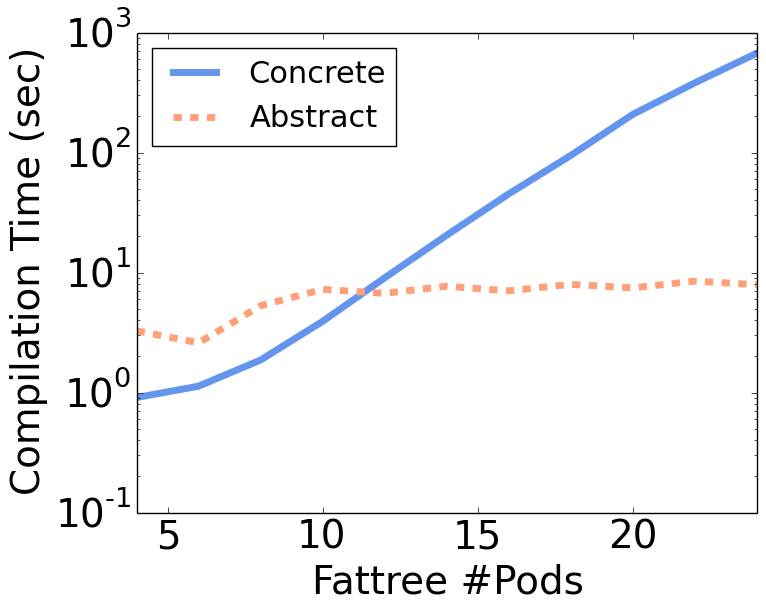
\includegraphics[width=.49\columnwidth]{figures/Fattree-time.png}}
  \subcaptionbox{Backbone}
    {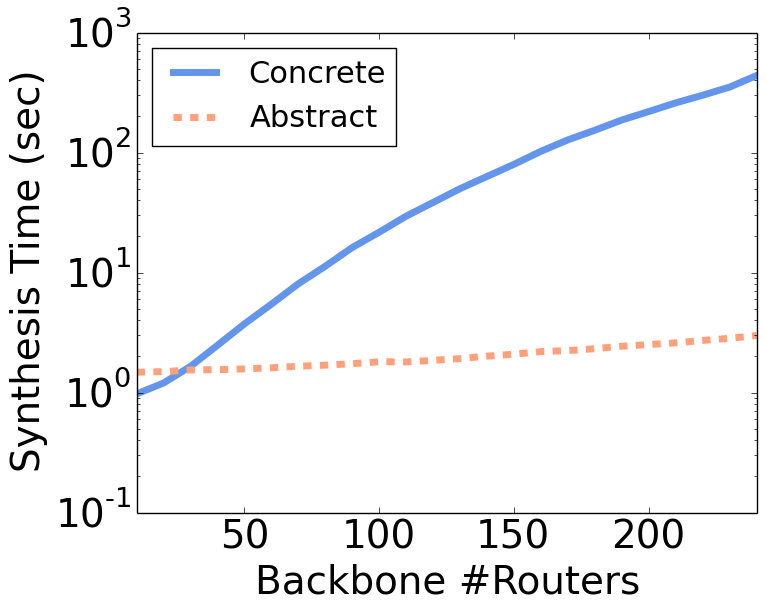
\includegraphics[width=.49\columnwidth]{figures/backbone-time.png}} \\
  \caption{Concrete vs. Abstract Compilation Time. \label{fig:compilation-times}}
  \vspace{-1em}
\end{figure}

\begin{figure}[t!]
  \subcaptionbox{Datacenter}
    {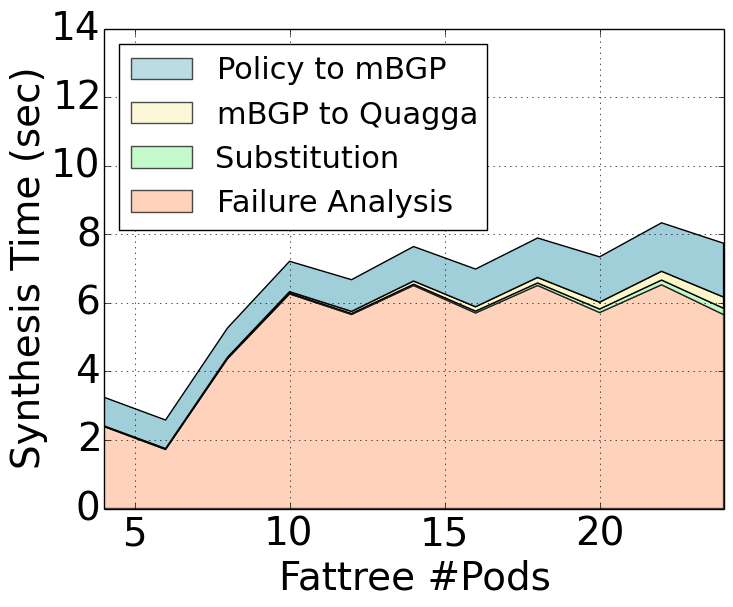
\includegraphics[width=.49\columnwidth]{figures/Fattree-analysis-time.png}}
  \subcaptionbox{Backbone}
    {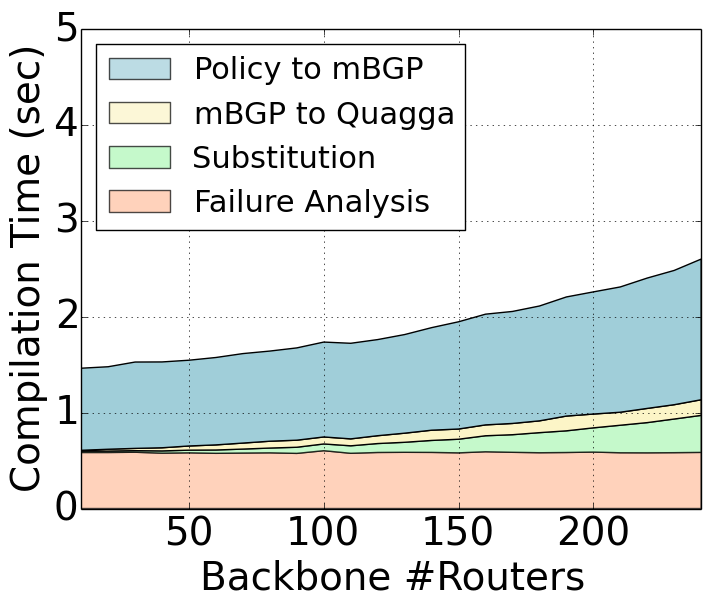
\includegraphics[width=.49\columnwidth]{figures/backbone-analysis-time.png}} \\
  \caption{Abstract Compilation Time by Phase. \label{fig:abstract-breakdown}}
  \vspace{-1em}
\end{figure}

Using abstraction allows us to naturally scale network synthesis in \sysname. We evaluate compilation time in \sysname both with and without abstraction using routing policy for backbone and datacenter networks inspired by configurations obtained from a large cloud provider.

\para{Routing Policy}

Routers in the datacenter network run BGP using private AS numbers and peer with each other and with the backbone network over eBGP. The routers aggregate some prefix blocks when announcing them to the backbone network, and they keep some prefixes internal. The policy also ensures bogons and private address space from external neighbors is dropped. The data center prefers that traffic leave through certain peers over others and ensures that transit traffic between peers is never allowed in the datacenter.

The backbone network classifies external neighbors into several different categories based on commercial relationship and prefers paths through them in order. Similar to the datacenter, it prevents bogons and private address space from external neighbors, drops transit traffic between certain peers but not through others, and aggregates internal prefixes at the border of the network.

\para{Network Topology}

For both networks, we use the same routing policy but scale the size of the underlying topology. For the datacenter networks, we use a standard Fat Tree topology and scale the size of the topology according the the number of pods $k$, starting with 4 pods and ending with 24 pods. The abstract topology uses a single abstract node for each tier of the datacenter, an additional abstract node for tier 0 to separate local and global prefixes, as well as a single abstract node for each group of equivalent eBGP neighbor.

For the backbone networks, we split the network into two parts: a collection of border routers and a fully-connected internal core. We scale the backbone networks from 10 to 250 routers. The abstract topology uses a single abstract node for the network border routers and another abstract node for the network core. Backbone eBGP-speaking peers are grouped into abstract nodes based on their commercial relationship to the current AS (e.g., customer, provider, peer).

\para{Results}

Figure~\ref{fig:compilation-times} shows compilation time for the same policies for both the abstract and concrete versions of the policies described above. All experiments are run on an 8 core, 2.4 GHz Intel i7 processor Mac with 8GB of Ram.

For both the datacenter and backbone networks, the abstract compilation starts off slightly slower than concrete compilation for small topologies due to the overhead of the abstract k-disjoint path analysis for aggregation black-hole safety. However, as the size of the topology increases, abstract compilation becomes orders of magnitude faster than concrete compilation. In all cases for both networks, abstract compilation takes less than 10 seconds to complete.

Figure~\ref{fig:abstract-breakdown} shows the relative time taken by each phase of abstract compilation. Notably, the abstract analysis takes the majority of the time, however the analysis does not depend on the number of concrete nodes in the network, and thus is largely a fixed cost. In particular, the number of calls to Z3 remains constant the across topology size. The seesaw behavior for the data center networks results from differences in time taken by Z3 to minimize the same constraints with different parameters.




%=====================================================
%
%
%  **Related Work**
%
%
%=====================================================

\section{Related Work}
\label{sec:related}

\begin{easylist}[itemize]
& Topologies: DCell, BCube, Fattree, ...
& Topology Abstraction: Condor
& Memory Shape Analysis: Sagiv, others
& Configuration automation
& Configuration analysis
& Configuration synthesis
\end{easylist}

%Our work draws on four threads of prior work.%

%\para{Topology abstraction}%

%\para{Topology design}%

%\para{Configuration automation}
%Many practitioners use configuration templates~\cite{hatch,thwack}, to ensure certain kinds of consistency across similar devices. In addition, configuration languages such as RPSL~\cite{RFC2622}, Yang~\cite{RFC6020}, and Netconf~\cite{RFC6241} allow operators to express routing policy in a vendor-neutral way.
%However, all of these solutions remain low-level, for example, requiring operators to specify exact local preferences. Unlike \sysname, there is no guarantee that these low-level configurations satisfy the original, high-level intent.%

%\para{Configuration analysis}
%The notion that configuring network devices is difficult and error-prone is not new.
%In the past, researchers have tried to tackle this problem by analyzing existing
%router configurations~\cite{feamster+:rcc,ipassure,batfish,bagpipe,arc} and reporting errors or inconsistencies when they are detected.
%Our research is complementary to these analysis
%efforts.  We hope to eliminate bugs by using higher-level
%languages and a ``correct-by-construction''
%methodology. Writing configurations at a high level of abstraction simplifies policy implementation and prevents a whole host of low-level errors.%

%\para{Configuration synthesis}
%ConfigAssure~\cite{narain:lisa05,narain+:configassure}
%is another system designed to
%help users define and debug low-level router
%configurations.  Inputs to
%ConfigAssure include a \emph{configuration database}, which contains a
%collection of tuples over constants and configuration variables, and a
%\emph{requirement}, which is a set of constraints.
%%
%The authors use a combination of logic programming and
%SAT solving to find concrete values for configuration variables.
%ConfigAssure handles configuration for a wide range of protocols and many
%different concerns.  In contrast, the scope of \sysname is much
%narrower.  In return, \sysname offers compact, higher-level
%abstractions customized for our domain, such as regular paths, as well
%as domain-specific analyses customized to those abstractions, such as
%our failure safety analysis.  The implementation technology is also
%entirely different, as we define algorithms over automata and graphs
%as opposed to using logic programming and SAT-based model-finding.



%=====================================================
%
%
%  **Conclusions**
%
%
%=====================================================

\section{Conclusions}
\label{sec:conclusions}



\para{Acknowledgments}




%=====================================================
%
%
%  **Bibliography**
%
%
%=====================================================

\balance

\bibliographystyle{abbrv}
\bibliography{references}


%=====================================================
%
%
%  **Appendix**
%
%
%=====================================================

\appendix

\begin{figure*}[t]\small
  \begin{minipage}[t]{.45\linewidth}
  \hdr{Syntax}{}
  \vspace*{-1\baselineskip}
  %
  \[ \begin{array}{rclr}
    \hline%

     pol     &::=& p_1, \dots, p_n & \textit{policies} \\
     p       &::=& t \hspace{.3em} \Path \hspace{.3em} r_1 \Prefer \dots \Prefer r_m \BNFALT cc & \textit{constraints} \\
     x       &::=& d.d.d.d/d & \textit{prefix} \\
     t       &::=& \True & \textit{true} \\
         &\BNFALT& \neg t & \textit{negation} \\
         &\BNFALT& t_1 \vee t_2 & \textit{disjunction} \\
         &\BNFALT& t_1 \wedge t_2 & \textit{conjunction} \\
         &\BNFALT& \textit{prefix} = x & \textit{prefix test} \\
     r       &::=& l & \textit{location} \\
         &\BNFALT& \emptyset & \textit{empty set} \\
         &\BNFALT& \In & \textit{internal loc} \\
         &\BNFALT& \Out & \textit{external loc} \\
         &\BNFALT& r_1 \cup r_2 & \textit{union} \\
         &\BNFALT& r_1 \cap r_2 & \textit{intersection} \\
         &\BNFALT& r_1 \cdot r_2 & \textit{concatenation} \\
         &\BNFALT& \NOT r & \textit{path negation} \\
         &\BNFALT& r^* & \textit{iteration} \\
     cc     &::=& agg(x, r_1 \rightarrow r_2)  & \textit{control constraints} \\
  \end{array} \]%

  \end{minipage}
  %
  ~~
  \vrule
  ~~
  %
  \begin{minipage}[t]{.5\linewidth}\small
  \hdr{Propane Expansions}{}
  \vspace*{-1\baselineskip}
  %
  \[\begin{array}{rcl}
    \hline
    \Any               & = & \Sigma^* \\
    \None              & = & \emptyset \\
    \Internal          & = & \In^+ \\
    \Always(X)         & = & X^* \\
    \Never(X)          & = & (!X)^* \\
    \Through(X)        & = & \Sigma^* \cdot X \cdot \Sigma^* \\
    \Eventually(X)     & = & \Out^* \cdot (X \cap \Out) \cdot \Out^* \cdot \In^+ \cdot \Out^* \\
    \Already(X)        & = & \Out^* \cdot \In^+ \cdot \Out^* \cdot (X \cap \Out) \cdot \Out^* \\
    \End(X)            & = & \Sigma^* \cdot X \\
    \Start(X)          & = & X \cdot \Sigma^* \\
    \Enter(X)          & = & \Sigma^* \cdot \Out \cdot (X \cap \In) \cdot \Sigma^* ~ \cup \\
                       &   & \Sigma^* \cdot (X \cap \Out) \cdot \In \cdot \Sigma^* \\
    \Exit(X)           & = & \Sigma^* \cdot \In \cdot (X \cap \Out) \cdot \Sigma^* ~ \cup \\
                       &   & \Sigma^* \cdot (X \cap \In) \cdot \Out \cdot \Sigma^* \\
    \LinkKW(X,Y)       & = & \Sigma^* \cdot X \cdot Y \cdot \Sigma^* \\
    \PathKW(\vec{X})   & = & \Sigma^* \cdot X_1 \dots X_n \cdot \Sigma^* \\
    \Novalley(\vec{X}) & = & \NOT\PathKW(X_2,X_1,X_2) ~ \cap \dots \cap \\
                       &   & \NOT\PathKW(X_n,X_{n-1},X_n) \\
  \end{array} \]%

  \end{minipage}%

  \hrulefill%

  \caption{Regular Intermediate Representation (RIR) syntax (left), and
           Propane language expansions (right).}
  \label{fig:rir-syntax}
  %\vspace{-1em}
\end{figure*}%





\end{document}
